\documentclass{beamer}
\usetheme{Amsterdam}
\usepackage{adjustbox}
\usepackage{graphicx}
\usepackage{subfig}
\graphicspath{{./figures/}{/Users/evayap/Documents/masters_thesis/presentation/TFL_WIP/plots/}{/Users/evayap/Documents/masters_thesis/presentation/masters_defence/figures/}{/Users/evayap/Documents/job_application/marra_presentation/figures/}}
% \usepackage{beamerthemesplit} // Activate for custom appearance
%\setbeamertemplate{caption}[numbered]
%\setbeamerfont{caption}{size=\scriptsize}
\usepackage{caption}
\captionsetup[figure]{labelformat=empty}
\captionsetup[table]{labelformat=empty}
\usepackage{siunitx}
\sisetup{range-phrase = \text{--}}
% create long tables that span multiple pages
\usepackage{longtable}

\addtobeamertemplate{navigation symbols}{}{%
    \usebeamerfont{footline}%
    \usebeamercolor[fg]{footline}%
    \hspace{1em}%
    \insertframenumber/\inserttotalframenumber
}

\setbeamercolor{footline}{fg=black}
%\setbeamerfont{footline}{series=\bfseries}

\setbeamertemplate{footnote}{%
  \tiny%
  \parindent 1em\noindent%
  \raggedright
  \hbox to 1.8em{\hfil\insertfootnotemark}\insertfootnotetext\par%
}%
\setlength\footnotesep{0pt}

\makeatletter
\def\blfootnote{\xdef\@thefnmark{}\@footnotetext}
\makeatother

\newcommand{\semitransp}[2][35]{\color{fg!#1}#2}

\title{Germline Variant Calling in Formalin-fixed Paraffin-embedded Tumours}
\author{Eva Yap, M.Sc. Student}
\date{Thesis defence -- Dec 12, 2017}

%%%%%%%%%%%%%%%%%%%%%%%%%%%%%%%%%%%%%%%%%%%%%%%%%%%%%%%%%%%%%%%%%%%%%
\begin{document}

\frame{\titlepage}

%Table of content
\begin{frame}
\frametitle{Overview}
\tableofcontents
\end{frame}

%Begin presentation
%Create overview page
\AtBeginSection[]
{
  \begin{frame}
    \frametitle{Overview}
    \tableofcontents[currentsection]
  \end{frame}
}

%%%%%%%%%%%%%%%%%%%%%%%%%%%%%%%%%%%%%%%%%%%%%%%%%%%%%%%%%%%%%%%%%%%%%
% Background
\section{Background}
%%%%%%%%%%%%%%%%%%%%%%%%%%%%%%%%%%%%%%%%%%%%%%%%%%%%%%%%%%%%%%%%%%%%%

\begin{frame}
\frametitle{Cancer is a leading cause of death in Canada}
\centering
\vspace{-4mm}
\begin{figure}[t]
    \includegraphics[scale=0.4]{cancer_stats.png}
\end{figure}
\vspace{-4mm}
\only<2>{In 2017, the estimate number of new cancer cases is 206,200 and deaths from cancer is 80,800.}
\blfootnote{Canadian Cancer Society's Advisory Committee on Cancer Statistics, 2017. Canadian Cancer Society.}
\end{frame}

\begin{frame}
\frametitle{Genomic-driven cancer medicine has great potential in guiding oncologic care}
\centering
\vspace{-4mm}
\begin{figure}[t]
    \includegraphics[scale=0.24]{genomic_cancer_medicine.png}
\end{figure}
\blfootnote{S. Roychowdhury \& A.M. Chinnaiyan, 2014. Annu. Rev. Genomics Hum. Genet, 15:395-415.}
\blfootnote{H. Mano, 2015. Proc. Jpn. Acad. Ser. B. Phys. Biol. Sci, 91(5):193-201.}
\end{frame}

\begin{frame}
\frametitle{British Columbia Cancer Agency's OncoPanel}
\vspace{-4mm}
\begin{figure}[t]
    \includegraphics[scale=0.26]{oncopanel_amplicon_seq.png}
\end{figure}
\begin{enumerate}
\item Targeted amplicon-based next-generation sequencing panel for solid tumours
\item Detects single nucleotide variants (SNVs) and small indels in cancer- and pharmacogenomic-related genes
\end{enumerate}
\end{frame}

\begin{frame}
\frametitle{Germline variants can have clinical implications for both cancer patients and their families}
\begin{figure}[t]
    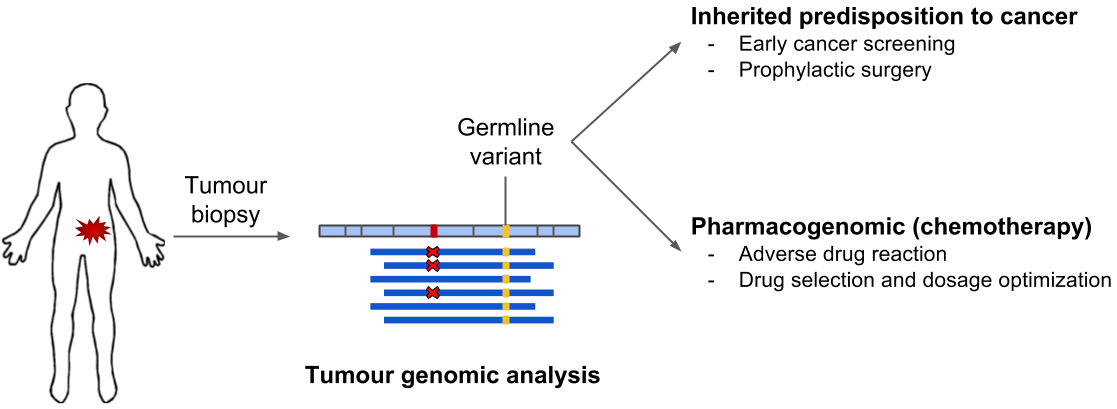
\includegraphics[scale=0.28]{germline_importance2.png}
\end{figure}
\end{frame}

\begin{frame}
\frametitle{\textit{UGT1A1} promoter polymorphism leads to irinotecan toxicity}
\begin{figure}[t]
    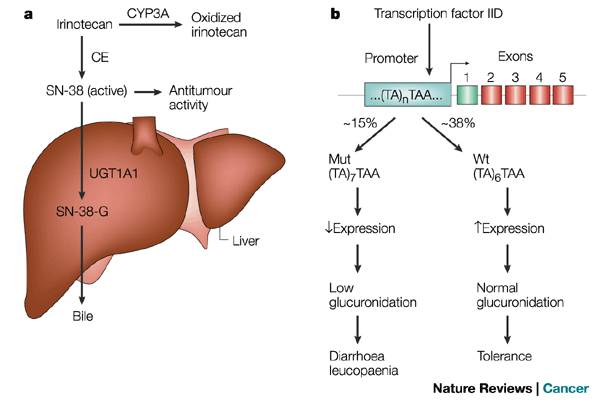
\includegraphics[scale=0.42]{ugt1a1.png}
\end{figure}
\blfootnote{M.V. Relling \& T. Dervieux, 2001. Nat. Rev. Cancer 1, 99-108}
\end{frame}

\begin{frame}
\frametitle{Germline variants can have clinical implications for both cancer patients and their families}
\begin{figure}[t]
    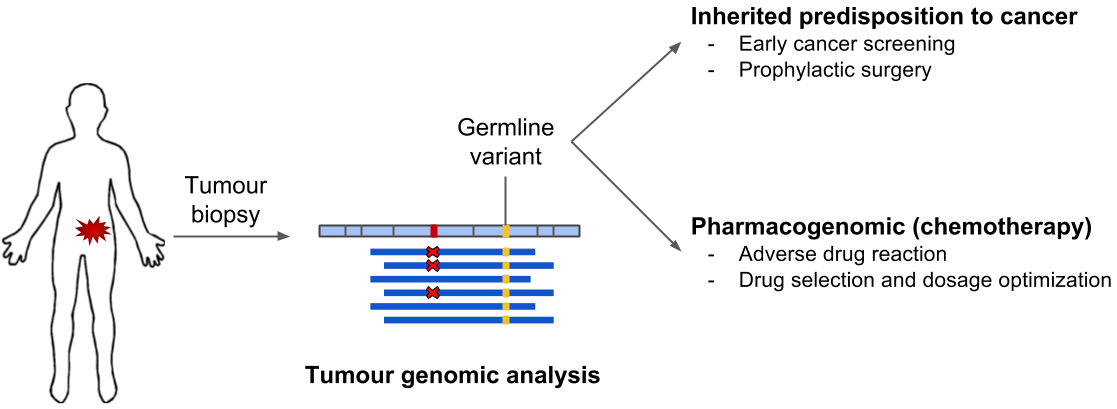
\includegraphics[scale=0.28]{germline_importance2.png}
\end{figure}
\centering
\textcolor{blue}{Reporting clinically important germline variants can improve clinical outcomes for both cancer patients and their families.}
\end{frame}

\begin{frame}
\frametitle{Clinical tumour sequencing presents an opportunity to pre-screen for germline variants}
\vspace{-6mm}
\begin{figure}[t]
    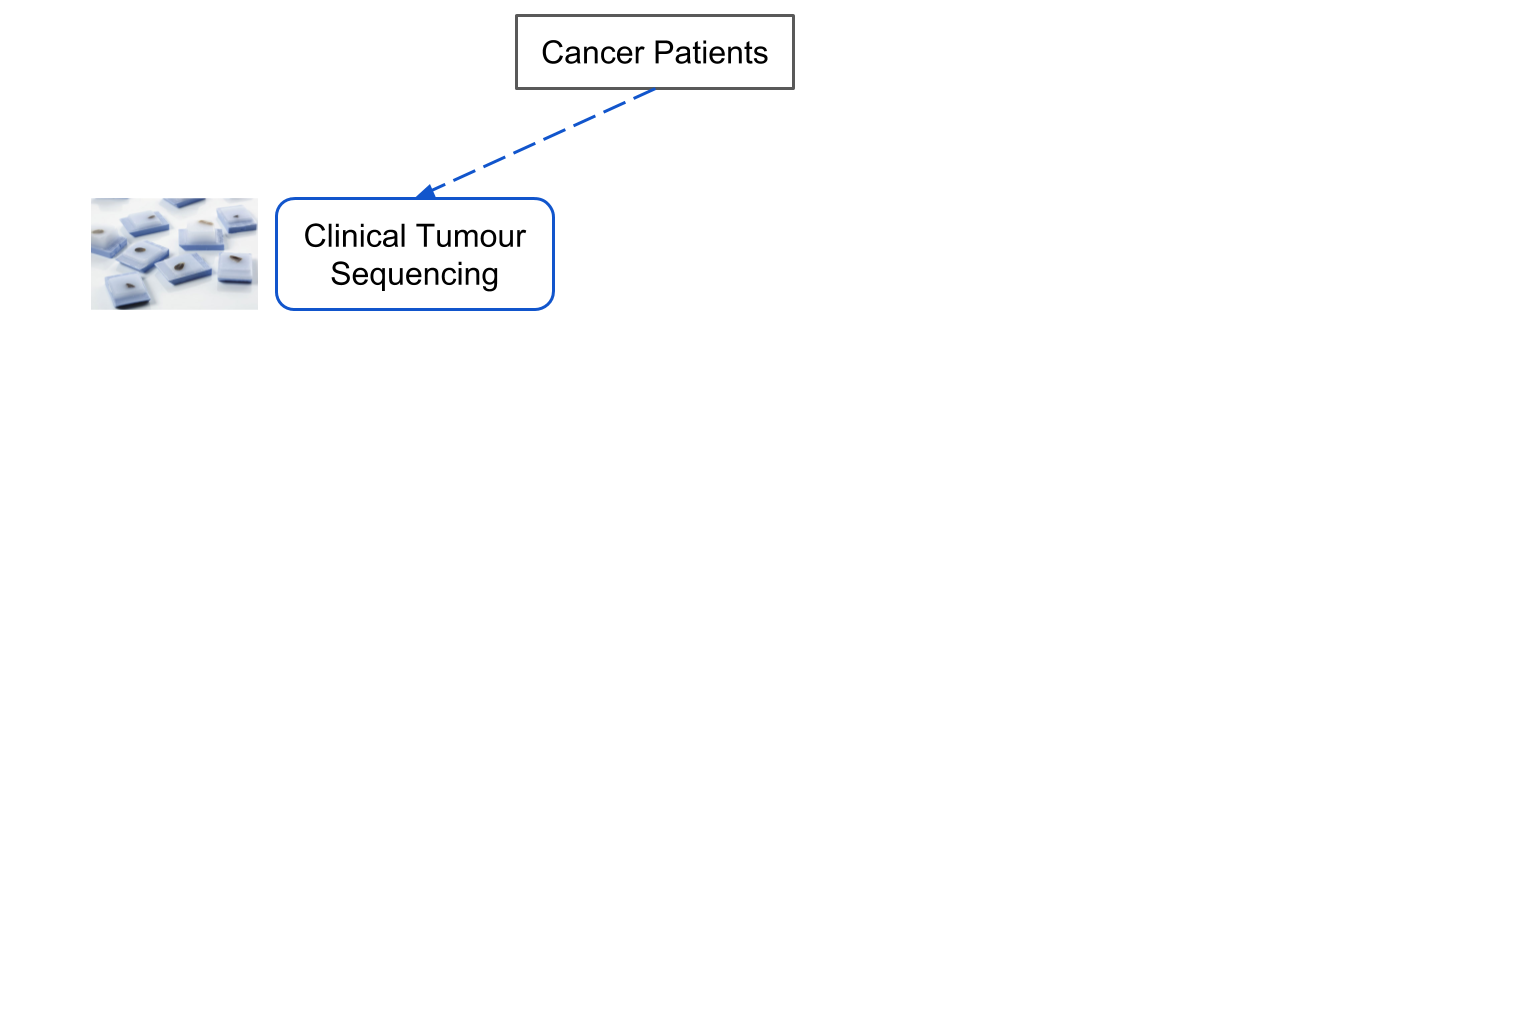
\includegraphics[scale=0.2]{opportunity_clinical_sequencing1a.png}
\end{figure}
\end{frame}

\begin{frame}
\frametitle{Clinical tumour sequencing presents an opportunity to pre-screen for germline variants}
\vspace{-6mm}
\begin{figure}[t]
    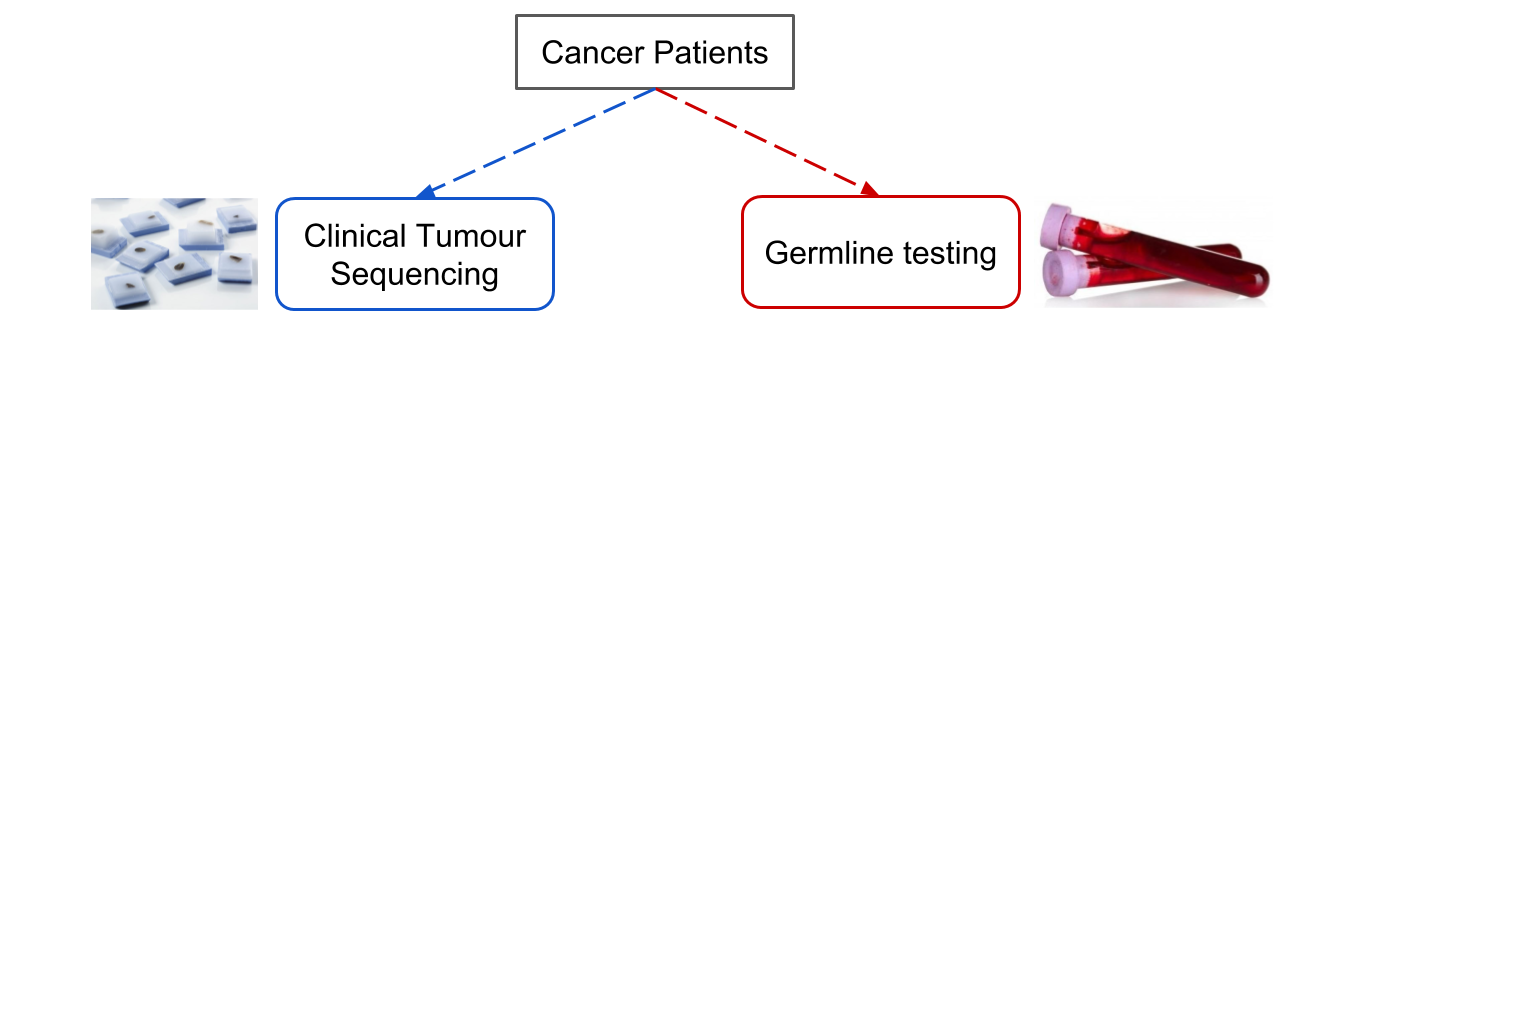
\includegraphics[scale=0.2]{opportunity_clinical_sequencing2a.png}
\end{figure}
\end{frame}

\begin{frame}
\frametitle{Clinical tumour sequencing presents an opportunity to pre-screen for germline variants}
\vspace{-6mm}
\begin{figure}[t]
    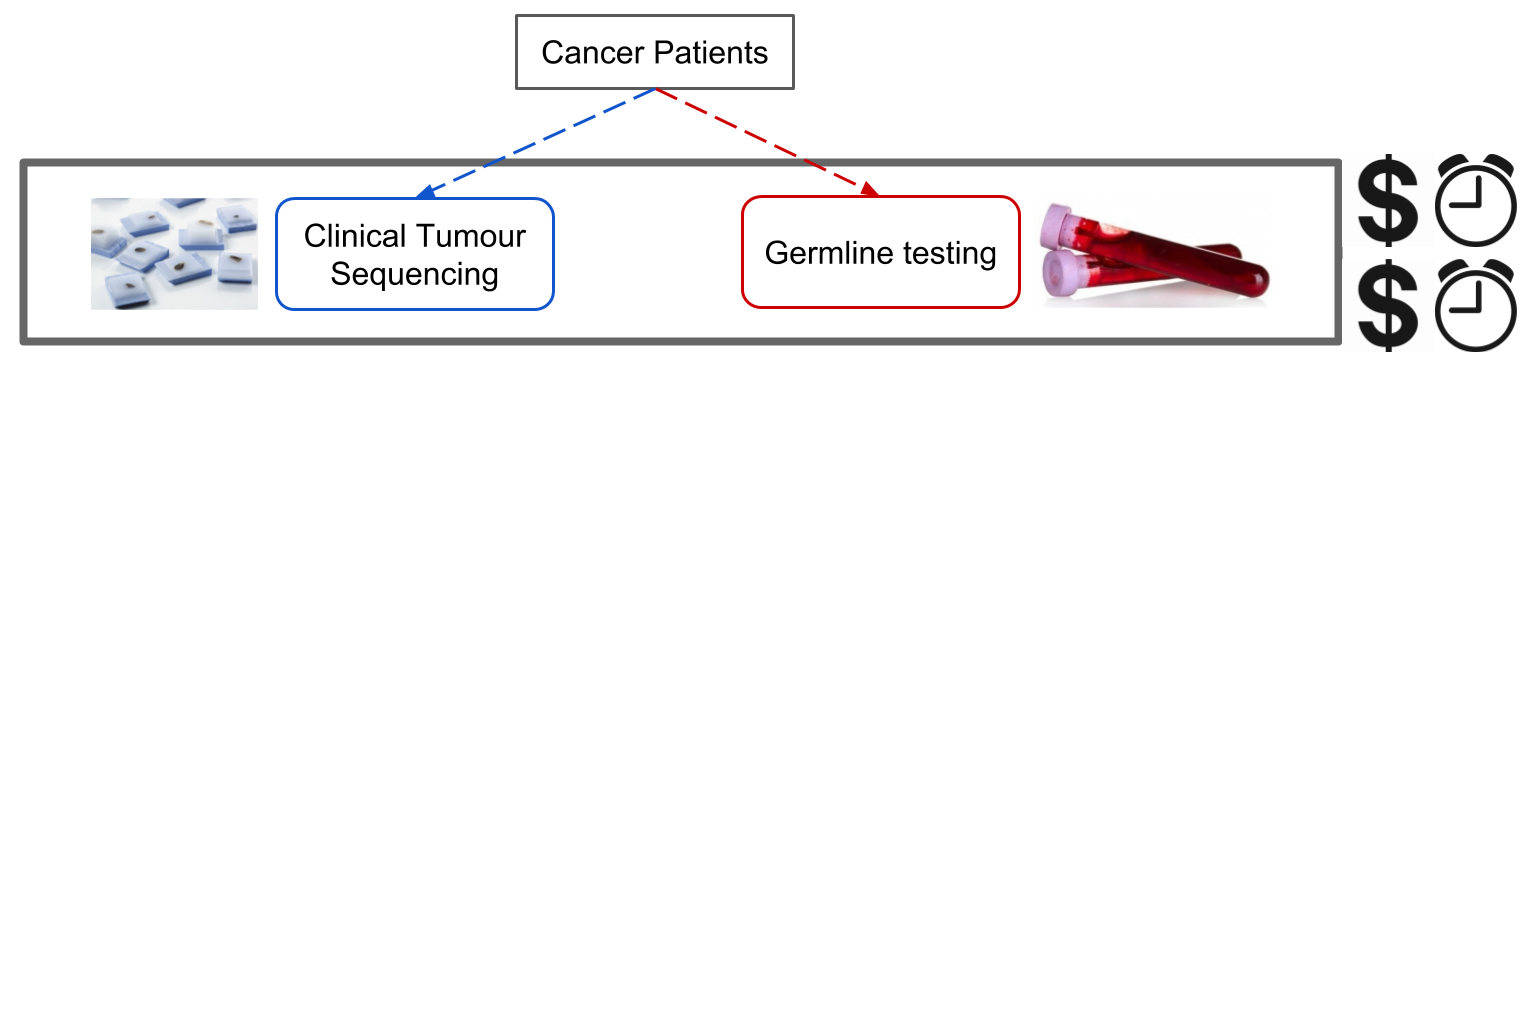
\includegraphics[scale=0.2]{opportunity_clinical_sequencing3a.png}
\end{figure}
\end{frame}

\begin{frame}
\frametitle{Clinical tumour sequencing presents an opportunity to pre-screen for germline variants}
\vspace{-6mm}
\begin{figure}[t]
    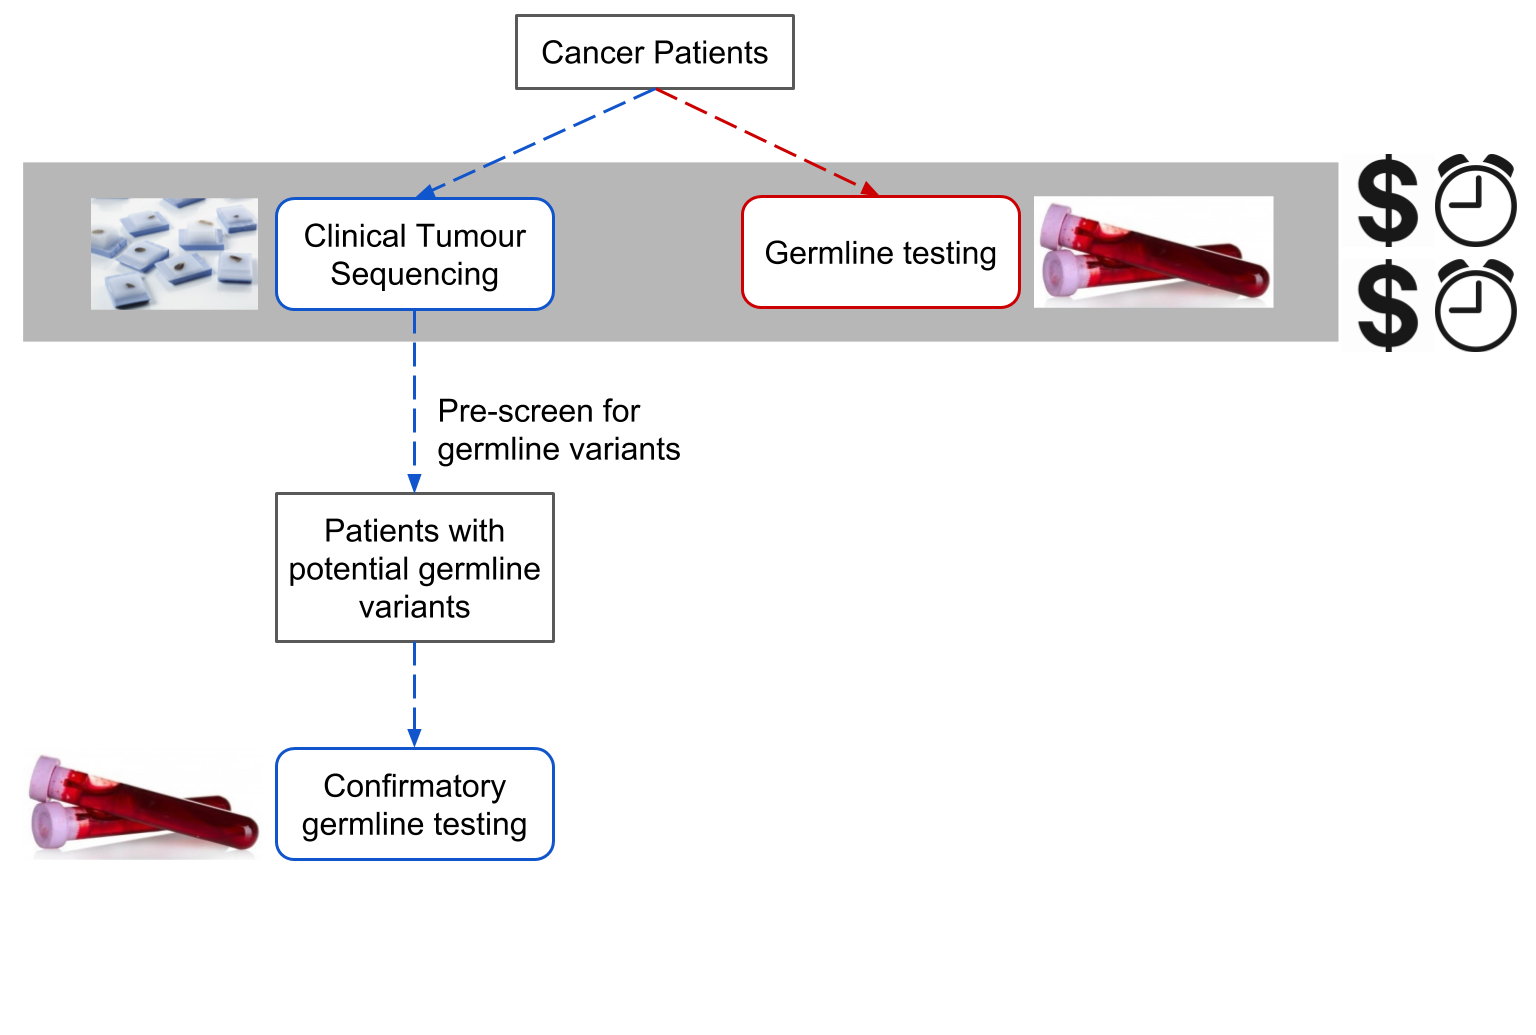
\includegraphics[scale=0.2]{opportunity_clinical_sequencing4a.png}
\end{figure}
\end{frame}

\begin{frame}
\frametitle{Clinical tumour sequencing presents an opportunity to pre-screen for germline variants}
\vspace{-6mm}
\begin{figure}[t]
    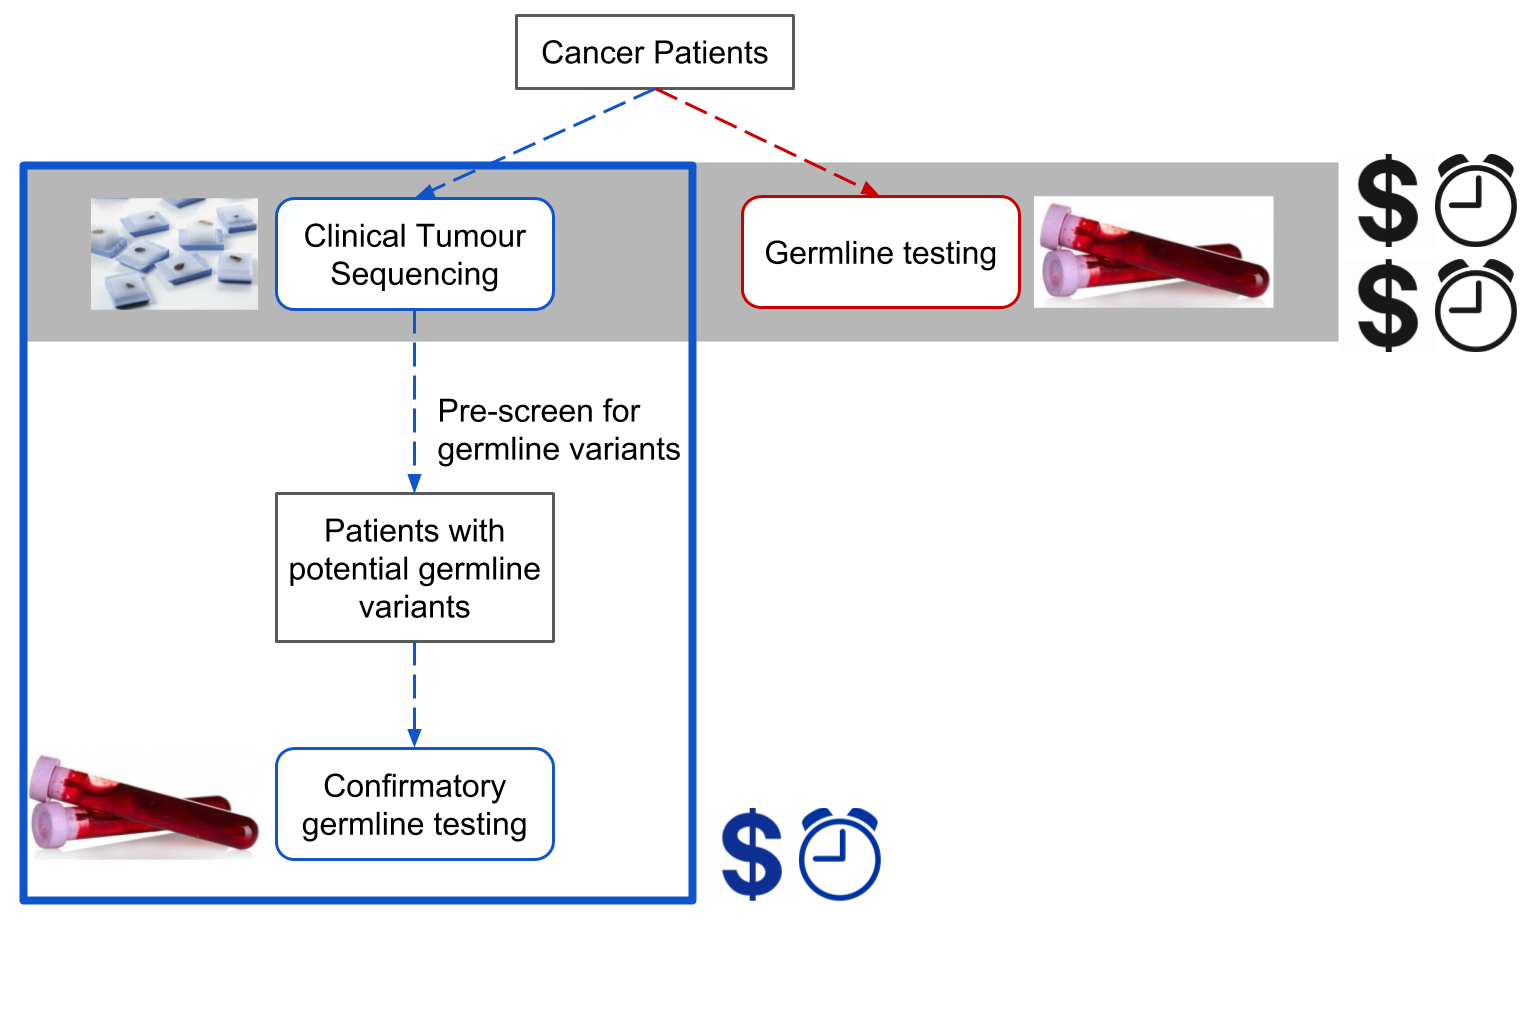
\includegraphics[scale=0.2]{opportunity_clinical_sequencing5a.png}
\end{figure}
\end{frame}

\begin{frame}
\frametitle{Challenges in identifying germline variants using clinical tumour-only sequencing}
\textbf{1}: Formalin-induced DNA damage
\begin{figure}[t]
    \includegraphics[scale=0.3]{ffpe_artifacts_review.png}
\end{figure}
\vspace{-2mm}
\begin{itemize}
\uncover<1->{\item Tumours are usually formalin-fixed and paraffin-embedded (FFPE) for pathologic assessment.}
\uncover<2->{\item Formaldehyde exposure causes fragmentation and sequence artifacts (e.g. C$>$T$/$G$>$A).}
\end{itemize}
\blfootnote{H. Do \& A. Dobrovic, 2015. Clin. Chem. 61(1): 64--71}
\end{frame}

\begin{frame}
\frametitle{Challenges in identifying germline variants using clinical tumour-only sequencing}
\textbf{2}: Distinguishing between germline and somatic variants
\begin{figure}[t]
    \includegraphics[scale=0.35]{distinguishing_somatic_germline_tumour.png}
\end{figure}
\end{frame}

\begin{frame}
\frametitle{Low accuracy in distinguishing between germline and somatic variants using \textcolor{blue}{unmatched normal sample} and \textcolor{red}{public databases}}
\vspace{-7mm}
\begin{figure}[t]
    \includegraphics[scale=0.35]{distinguishing_somatic_germline_jones1.png}
\end{figure}
\blfootnote{S. Jones, 2015. Sci. Transl. Med, 7(283):283ra53 (Fig. 3C)}
\end{frame}

\begin{frame}
\frametitle{Low accuracy in distinguishing between germline and somatic variants using \textcolor{blue}{unmatched normal sample} and \textcolor{red}{public databases}}
\vspace{-7mm}
\begin{figure}[t]
    \includegraphics[scale=0.35]{distinguishing_somatic_germline_jones2.png}
\end{figure}
\vspace{-5mm}
\centering
\only<2->{\textcolor{blue}{An approach to separate germline from somatic variants in FFPE tumour-only analyses must be established.}}
\blfootnote{S. Jones, 2015. Sci. Transl. Med, 7(283):283ra53 (Fig. 3C)}
\end{frame}

%%%%%%%%%%%%%%%%%%%%%%%%%%%%%%%%%%%%%%%%%%%%%%%%%%%%%%%%%%%%%%%%%%%%%
% Research question
\section{Research Question}
%%%%%%%%%%%%%%%%%%%%%%%%%%%%%%%%%%%%%%%%%%%%%%%%%%%%%%%%%%%%%%%%%%%%%

\begin{frame}
\frametitle{Research Question}
\begin{columns}[T] % align columns
\begin{column}{.48\textwidth}
\begin{figure}[t]
    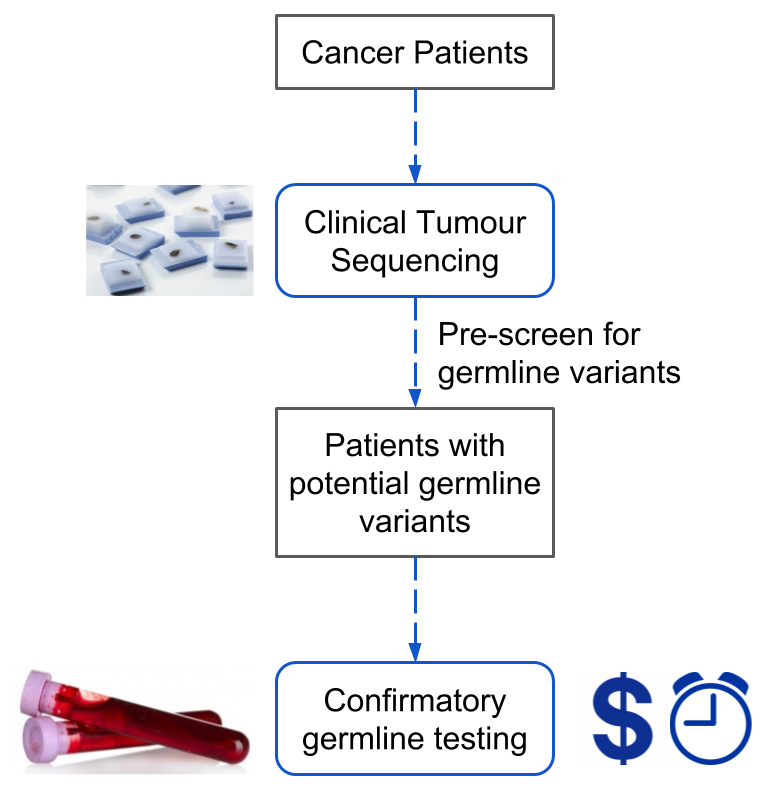
\includegraphics[scale=0.22]{opportunity_clinical_sequencing_research_question.png}
\end{figure}
\end{column}%
\hfill%
\begin{column}{.48\textwidth}
\uncover<2->{\textcolor{blue}{Can we use clinical tumour sequencing to identify germline variants?} \\~\\}
\uncover<3->{\textbf{Challenges:}}
\begin{itemize}
\uncover<3->{\item Formalin-induced DNA damage}
\uncover<3->{\item Distinguishing between germline and somatic variants}
\\~\\
\end{itemize}
\end{column}%
\end{columns}
\end{frame}

%%%%%%%%%%%%%%%%%%%%%%%%%%%%%%%%%%%%%%%%%%%%%%%%%%%%%%%%%%%%%%%%%%%%%
% Project aims
\section{Thesis Aims}
%%%%%%%%%%%%%%%%%%%%%%%%%%%%%%%%%%%%%%%%%%%%%%%%%%%%%%%%%%%%%%%%%%%%%

\begin{frame}
\frametitle{Thesis Aims}
\uncover<1->{\textcolor{blue}{Can we use clinical tumour sequencing to identify germline variants?}}
\\
\vspace{2mm}
\uncover<2->{\textbf{Challenge 1}: Formalin-induced DNA damage}
\\
\uncover<3->{\textcolor{blue}{Aim 1:} Characterize formalin-induced DNA damage in amplicon sequencing data}
\\
\vspace{2mm}
\uncover<4->{\textbf{Challenge 2}: Distinguishing between germline and somatic variants}
\\
\uncover<4->{\textcolor{blue}{Aim 2:} Determine the retention rate of germline variants in tumours}
\\
\uncover<5->{\textcolor{blue}{Aim 3:} Evaluate the use of variant allele frequency (VAF) thresholds to separate germline from somatic variants in FFPE tumours}
\end{frame}

\begin{frame}
\frametitle{Study Design: \textbf{T}he \textbf{O}ncoPanel \textbf{P}ilot (TOP) Study}
\begin{figure}[t]
    \includegraphics[scale=0.28]{study_design_general2.png}
\end{figure}
\end{frame}

\begin{frame}
\frametitle{Tumour types in the TOP cohort}
\small
\begin{table}
\caption{}
\centering
      \begin{tabular}{lccc}
        \hline
        Cancer Type & Number of Cases & Percentage (\%) \\ \hline
        Colorectal & 97 & 46 \\
        Lung & 59 & 28 \\
        Melanoma & 18 & 8 \\
				Other & 17 & 8 \\
				GIST & 7 & 3 \\
				Sarcoma & 4 & 2 \\
				Neuroendocrine & 4 & 2 \\
				Cervical & 2 & 0.9 \\
				Ovarian & 2 & 0.9 \\
				Breast & 2 & 0.9 \\
				Unknown & 1 & 0.5 \\
        \hline
      \end{tabular}
\end{table}
\end{frame}

\begin{frame}
\frametitle{Cancer-related genes in the OncoPanel}
\scriptsize
\begin{table}
    \caption{}
    \centering
    \begin{tabular}{lll}
    \hline
    Gene & Protein \\
    \hline
    AKT1 & Protein kinase B \\
    ALK & Anaplastic lymphoma receptor tyrosine kinase \\
    BRAF & Serine/threonine-protein kinase B-Raf \\
    EGFR & Epidermal growth factor receptor \\
    HRAS & GTPase HRas \\
    MAPK1 & Mitogen-activated protein kinase 1 \\
    MAP2K1 & Mitogen-activated protein kinase kinase 1 \\
    MTOR & Serine/threonine-protein kinase mTOR \\
    NRAS & Neuroblastoma RAS viral oncogene homolog \\
    PDGFRA & Platelet-derived growth factor receptor alpha \\
    PIK3CA & Phosphatidylinositol-4,5-bisphosphate 3-kinase catalytic subunit alpha \\
    PTEN & Phosphatase and tensin homolog \\
    STAT1 & Signal transducer and activator of transcription 1 \\
    STAT3 & Signal transducer and activator of transcription 3 \\
    TP53 & Tumor protein P53 \\
    \hline
    \end{tabular}
\end{table}
\end{frame}

\begin{frame}
\frametitle{Pharmacogenomic-related genes in the OncoPanel}
\scriptsize
\begin{table}
    \caption{}
    \centering
    \begin{tabular}{llll}
    \hline
    Gene & Protein & Chemotherapy \\
    \hline
    DPYD & Dihydropyrimidine dehydrogenase & 5-FU \\
    GSTP1 & Glutathione S-transferase pi 1 & Oxaliplatin \\
    MTHFR & Methylenetetrahydrofolate reductase & 5-FU \\
    TYMP & Thymidine phosphorylase & 5-FU \\
    TYMS & Thymidylate synthetase & 5-FU \\
    UGT1A1 & Uridine diphosphate (UDP)-glucuronosyl transferase 1A1 & Irinotecan \\
    \hline
    \end{tabular}
\end{table}
\end{frame}

%%%%%%%%%%%%%%%%%%%%%%%%%%%%%%%%%%%%%%%%%%%%%%%%%%%%%%%%%%%%%%%%%%%%%
% Project Aim 1
\section[Aim 1]{Aim 1: Formalin-induced DNA damage could be mitigated by using shorter amplicons and avoiding older FFPE blocks.}
%%%%%%%%%%%%%%%%%%%%%%%%%%%%%%%%%%%%%%%%%%%%%%%%%%%%%%%%%%%%%%%%%%%%%

\begin{frame}
\frametitle{Aim 1: Characterize formalin-induced DNA damage in amplicon sequencing data}
\begin{figure}[t]
    \includegraphics[scale=0.25]{study_design_aim1.png}
\end{figure}
\end{frame}

%%%%%%%%%%%%%%%%%%%%%%%%%%%%%%%%%%%%%%%%%%%%%%%%%%%%%%%%%%%%%%%%%%%%%
\begin{frame}
\frametitle{Formalin-induced DNA fragmentation could affect amplicon enrichment}
\begin{figure}[t]
    \includegraphics[scale=0.3]{fragmentation_amp_enrichment.png}
\end{figure}
\end{frame}

%%%%%%%%%%%%%%%%%%%%%%%%%%%%%%%%%%%%%%%%%%%%%%%%%%%%%%%%%%%%%%%%%%%%%
\begin{frame}
\frametitle{FFPE specimens demonstrate reduced amplicon enrichment}
\begin{figure}[t]
    \begin{columns}
    \column{5cm}
    \centering
    Enrichment efficiency:
    \[
    log2\frac{\text{Amplicon Yield (ng)}}{\text{DNA Input (ng)}}
    \]%
    \column{7cm}
    \centering
    \includegraphics[scale=0.65]{amplicon_enrichment_xlabel.png}
    \end{columns}
\end{figure}
\end{frame}

%%%%%%%%%%%%%%%%%%%%%%%%%%%%%%%%%%%%%%%%%%%%%%%%%%%%%%%%%%%%%%%%%%%%%
\begin{frame}
\frametitle{Formalin-induced DNA damage could affect read alignments}
\begin{figure}[t]
    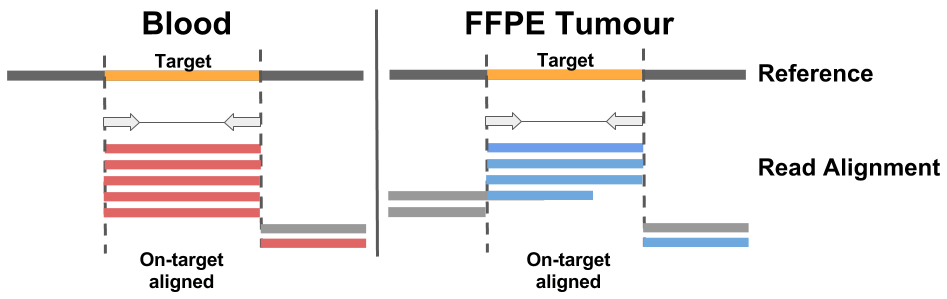
\includegraphics[scale=0.32]{ontarget_aligned.png}
\end{figure}
\end{frame}

%%%%%%%%%%%%%%%%%%%%%%%%%%%%%%%%%%%%%%%%%%%%%%%%%%%%%%%%%%%%%%%%%%%%%
\begin{frame}
\frametitle{FFPE and blood specimens show comparable percentage of on-target aligned reads}
\begin{figure}[t]
    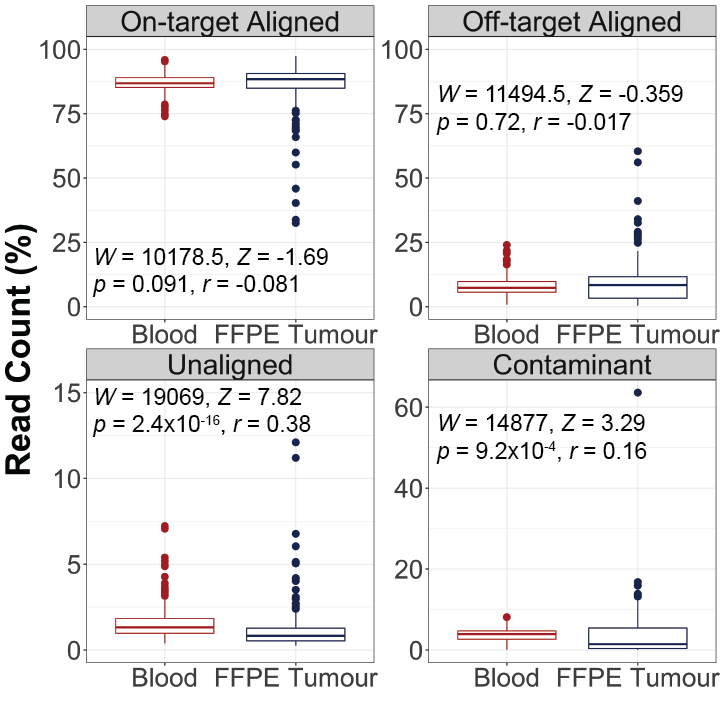
\includegraphics[scale=0.52]{alignment_pct.png}
    \vspace{-4mm}
    \caption{\scriptsize Wilcoxon signed-rank test, \textit{p} $<$ 0.0001}
\end{figure}
\end{frame}

%%%%%%%%%%%%%%%%%%%%%%%%%%%%%%%%%%%%%%%%%%%%%%%%%%%%%%%%%%%%%%%%%%%%%
\begin{frame}
\frametitle{Measuring coverage uniformity as the percentage of target bases that met increasing coverage thresholds}
\begin{figure}[t]
    \includegraphics[scale=0.3]{coverage_uniformity.png}
\end{figure}
\end{frame}

%%%%%%%%%%%%%%%%%%%%%%%%%%%%%%%%%%%%%%%%%%%%%%%%%%%%%%%%%%%%%%%%%%%%%
\begin{frame}
\frametitle{FFPE specimen show lower coverage uniformity at coverage thresholds $>$100x}
\begin{figure}[t]
    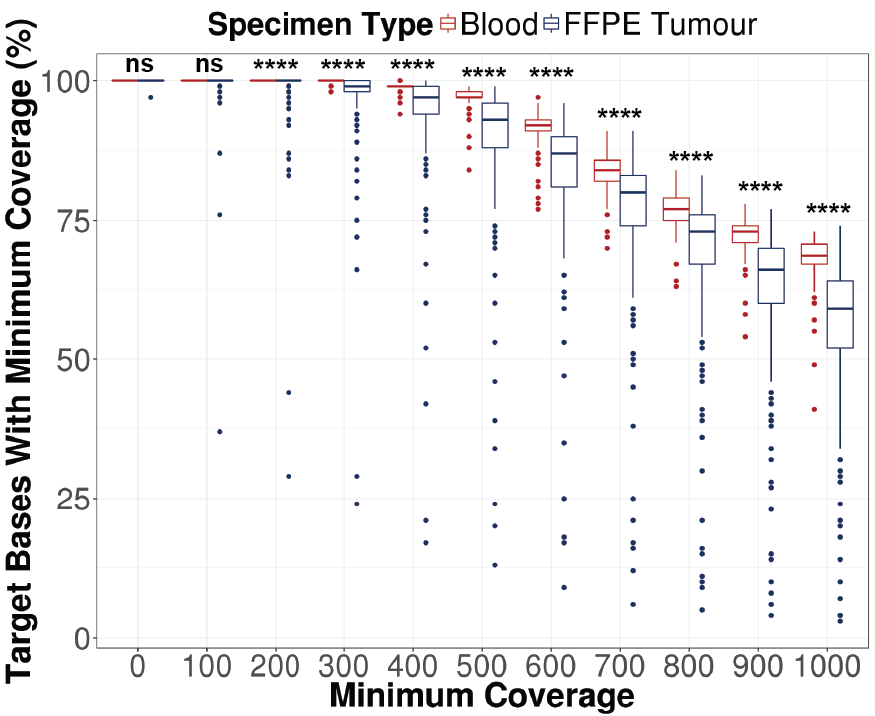
\includegraphics[scale=0.48]{coverage_stats_defence.png}
    \caption{\scriptsize Wilcoxon signed-rank test, ****\textit{p} $<$ 0.0001, ns = not significant}
\end{figure}
\end{frame}

%%%%%%%%%%%%%%%%%%%%%%%%%%%%%%%%%%%%%%%%%%%%%%%%%%%%%%%%%%%%%%%%%%%%%
\begin{frame}
\frametitle{OncoPanel consists of 416 amplicons}
\begin{figure}[t]
    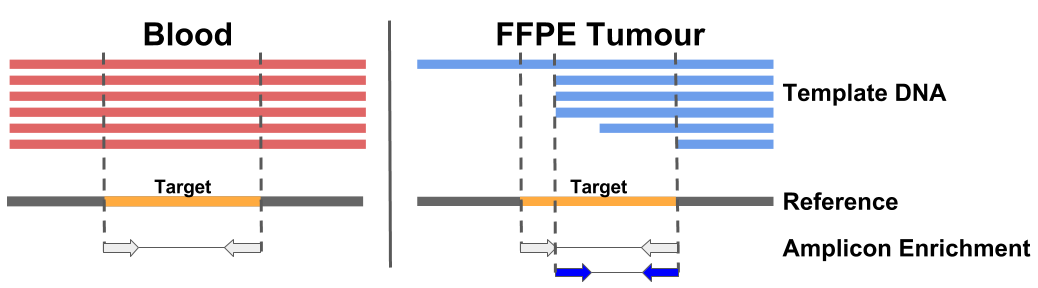
\includegraphics[scale=0.3]{amplicon_fragmentation.png}
\end{figure}
Shorter amplicons might yield greater coverage depth in FFPE specimens due to fragmentation damages in template DNA.
\end{frame}

%%%%%%%%%%%%%%%%%%%%%%%%%%%%%%%%%%%%%%%%%%%%%%%%%%%%%%%%%%%%%%%%%%%%%
\begin{frame}
\frametitle{Analysis of amplicon-specific coverage depth}
\begin{figure}[t]
    \includegraphics[scale=0.3]{amplicon_coverage2.png}
\end{figure}
Comparison of amplicon coverage was performed with the Wilcoxon signed-rank test.
\end{frame}

%%%%%%%%%%%%%%%%%%%%%%%%%%%%%%%%%%%%%%%%%%%%%%%%%%%%%%%%%%%%%%%%%%%%%
\begin{frame}
\frametitle{There are more amplicons with lower coverage depth in FFPE specimens relative to blood specimens}
\begin{figure}[t]
    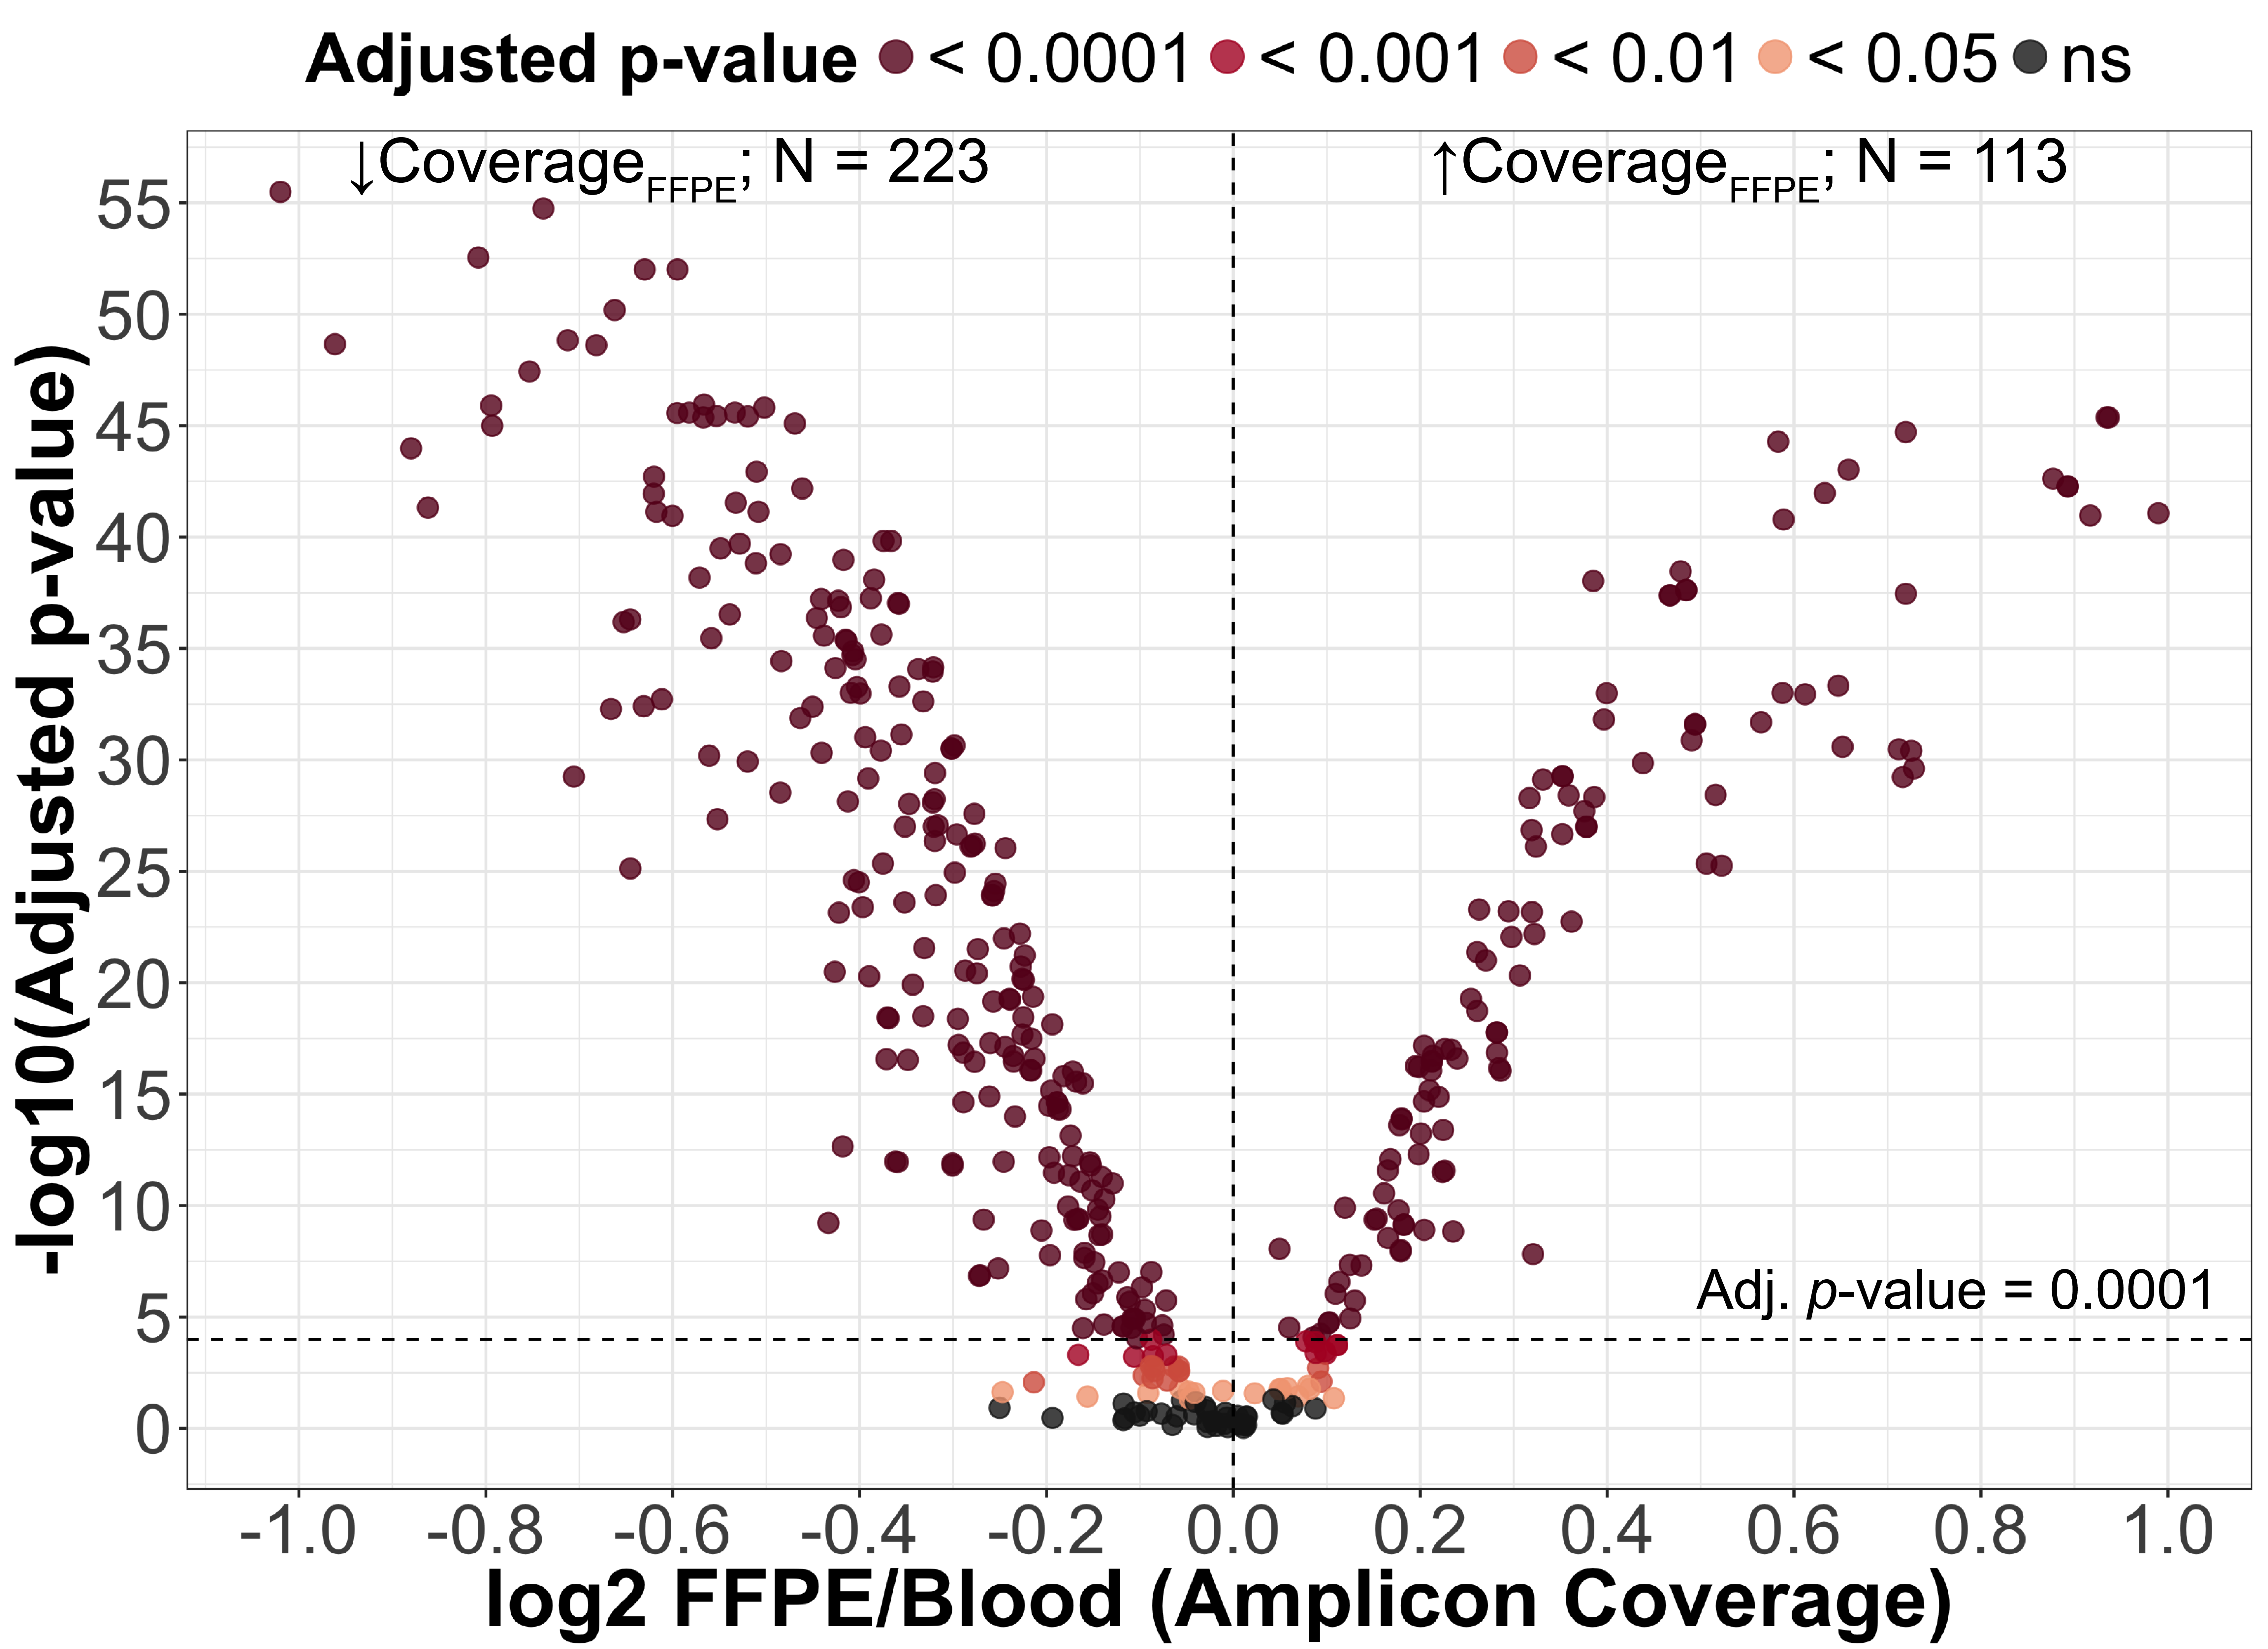
\includegraphics[scale=0.065]{amp_norm_depth_med_wilcoxon_volcano_85_xlabel.png}
    \caption{\scriptsize Wilcoxon signed-rank test with Benjamini Hochberg correction}
\end{figure}
\end{frame}

%%%%%%%%%%%%%%%%%%%%%%%%%%%%%%%%%%%%%%%%%%%%%%%%%%%%%%%%%%%%%%%%%%%%%
\begin{frame}
\frametitle{Decreased amplicon coverage in FFPE specimens is correlated with increased amplicon length and GC content}
\begin{figure}[t]
    \includegraphics[scale=0.5]{amp_cov_lm_len_gc_85_ylabel_remove_fig_lab.png}
    \caption{\scriptsize Pearson's correlation, \textit{p} $<$ 0.05}
\end{figure}
\end{frame}

%%%%%%%%%%%%%%%%%%%%%%%%%%%%%%%%%%%%%%%%%%%%%%%%%%%%%%%%%%%%%%%%%%%%%
\begin{frame}
\frametitle{Reduced amplicon coverage in FFPE specimens is more pronounced for longer amplicons}
\scriptsize
\begin{table}
\caption{Multiple regression of amplicon length and GC content as predictors for log2FC between amplicon coverage in FFPE specimens and blood.}
\label{multiple_regression}
\centering
      \begin{tabular}{l|ccccl}
        Variable & Unstandardized & S.E. & \textcolor{blue}{Standardized} & \textit{p}-value
        \\
        \hline
        Length (bp) & \num{-6.97e-3} & \num{2.59e-4} & \textcolor{blue}{\num{-7.56e-1}} & \num{7.45e-93}
				\\
				GC Content (\%) & \num{-1.03e-2} & \num{1.01e-3} & \textcolor{blue}{\num{-2.88e-1}} & \num{4.71e-22}
				\\
				\hline
				\\
				 & \multicolumn{4}{r}{Intercept = 1.63, Adjusted R\textsuperscript{2} = 0.673}
				\\
				 & \multicolumn{4}{r}{\textit{F}(2, 413) = 427.6, \textit{p}-value = \num{2.41e-101}}
				\\
				\hline
      \end{tabular} \\
\end{table}
\begin{enumerate}
\uncover<1->{\item 1 s.d. increase in amplicon length = \textcolor{blue}{0.756} s.d. decrease in log2FC}
\uncover<2->{\item 1 s.d. increase in amplicon GC content = \textcolor{blue}{0.288} s.d. decrease in log2FC}
\\~\\
\centering
\uncover<3->{\textcolor{blue}{Discrepancy in coverage depth between FFPE and blood specimens could be mitigated by using shorter amplicons.}}
\end{enumerate}
\end{frame}

%%%%%%%%%%%%%%%%%%%%%%%%%%%%%%%%%%%%%%%%%%%%%%%%%%%%%%%%%%%%%%%%%%%%%
\begin{frame}
\frametitle{FFPE specimens demonstrate increased C$>$T/G$>$A sequence artifacts}
\begin{figure}[t]
    \includegraphics[scale=0.58]{deamination_effect_blood_ffpe2.png}
    \caption{\scriptsize Wilcoxon signed-rank, \textit{p} $<$ 0.0001}
\end{figure}
\end{frame}

%%%%%%%%%%%%%%%%%%%%%%%%%%%%%%%%%%%%%%%%%%%%%%%%%%%%%%%%%%%%%%%%%%%%%
\begin{frame}
\frametitle{Increased age of paraffin block results in lower amplicon enrichment}
\begin{figure}[t]
    \includegraphics[scale=0.55]{deamination_effect_age_amp_yield_ylabel2.png}
    \caption{\scriptsize Spearman's rank correlation, \textit{p} $<$ 0.05}
\end{figure}
\end{frame}

%%%%%%%%%%%%%%%%%%%%%%%%%%%%%%%%%%%%%%%%%%%%%%%%%%%%%%%%%%%%%%%%%%%%%
\begin{frame}
\frametitle{Increased age of paraffin block results in elevated events of C$>$T/G$>$A sequence artifacts}
\vspace{-2mm}
\begin{figure}[t]
    \includegraphics[scale=0.45]{deamination_effect_age2.png}
    \vspace{-2mm}
    \caption{\scriptsize Spearman's rank correlation, \textit{p} $<$ 0.05}
\end{figure}
\end{frame}

%%%%%%%%%%%%%%%%%%%%%%%%%%%%%%%%%%%%%%%%%%%%%%%%%%%%%%%%%%%%%%%%%%%%%
\begin{frame}
\frametitle{Summary for Aim 1}
\begin{enumerate}
\uncover<1->{\item FFPE specimens demonstrated reduced amplicon enrichment.}
\uncover<2->{\item FFPE and blood specimens showed comparable percentage of on-target aligned reads.}
\uncover<3->{\item Discrepancy in coverage depth between blood and FFPE specimens was more pronounced for longer amplicons.}
\\~\\
\uncover<4->{\textcolor{blue}{Recommendation: Use shorter amplicons}}
\end{enumerate}
\end{frame}

\begin{frame}
\frametitle{Summary for Aim 1}
\begin{enumerate}
\setcounter{enumi}{3}
\uncover<1->{\item Increased C$>$T/G$>$A and A$>$G/T$>$C artifacts were observed in FFPE specimens, but these differences were minor.}
\uncover<2->{\item Increased age of paraffin block resulted in lower amplicon enrichment and elevated events of artifactual transitions.}
\\~\\
\uncover<3->{\textcolor{blue}{Recommendation: Avoid long-term storage of FFPE blocks}}
\end{enumerate}
\end{frame}

%%%%%%%%%%%%%%%%%%%%%%%%%%%%%%%%%%%%%%%%%%%%%%%%%%%%%%%%%%%%%%%%%%%%%
% Project Aim 2
\section[Aim 2]{Aim 2: FFPE tumour DNA is a reliable source for germline variant calling.}
%%%%%%%%%%%%%%%%%%%%%%%%%%%%%%%%%%%%%%%%%%%%%%%%%%%%%%%%%%%%%%%%%%%%%

\begin{frame}
\frametitle{Aim 2: Determine the retention rate of germline variants in tumours}
\centering
\begin{figure}[t]
    \includegraphics[scale=0.25]{study_design_aim2.png}
\end{figure}
\end{frame}

\begin{frame}
\frametitle{Variant analysis pipeline}
\centering
\begin{figure}[t]
    \includegraphics[scale=0.22]{variant_analysis_pipeline.png}
\end{figure}
\end{frame}

\begin{frame}
\frametitle{Eight drug-response-related germline variants are identified with the ClinVar database}
\centering
\begin{table}
\centering
      \begin{tabular}{l|lll}
      \hline
      Gene & Variant & dbSNP ID & Frequency\textsuperscript{$\dagger$}
      \\
      \hline
      TP53 & p.Arg72Pro$/$c.215G$>$C & rs1042522 & 97
      \\
      DPYD & p.Asp949Val$/$c.2846A$>$T & rs67376798 & 2
      \\
       & c.1906G$>$A & rs3918290 & 1
      \\
       & p.Met166Val$/$c.496A$>$G & rs2297595 & 34
      \\
      GSTP1 & p.Ile105Val$/$c.313A$>$G & rs1695 & 109
      \\
      MTHFR & p.Glu429Ala$/$c.1286A$>$C & rs1801131 & 102
      \\
       & p.Ala222Val$/$c.665C$>$T & rs1801133 & 110
      \\
      TYMS & c.\*447\_\*452delTTAAAG & rs151264360 & 132
      \\
      \hline
      \end{tabular}
    \end{table}
    \footnotesize\textsuperscript{$\dagger$}Out of 213 patients.
\end{frame}

\begin{frame}
\frametitle{Eight drug-response-related germline variants are identified with the ClinVar database}
\centering
\begin{table}
\centering
      \begin{tabular}{l|lll}
      \hline
      Gene & Variant & dbSNP ID & Frequency\textsuperscript{$\dagger$}
      \\
      \hline
      TP53 & p.Arg72Pro$/$c.215G$>$C & rs1042522 & 97
      \\
      DPYD & p.Asp949Val$/$c.2846A$>$T & rs67376798 & 2
      \\
       & \textcolor{blue}{c.1906G$>$A} & \textcolor{blue}{rs3918290} & \textcolor{blue}{1}
      \\
       & p.Met166Val$/$c.496A$>$G & rs2297595 & 34
      \\
      GSTP1 & p.Ile105Val$/$c.313A$>$G & rs1695 & 109
      \\
      MTHFR & p.Glu429Ala$/$c.1286A$>$C & rs1801131 & 102
      \\
       & p.Ala222Val$/$c.665C$>$T & rs1801133 & 110
      \\
      TYMS & c.\*447\_\*452delTTAAAG & rs151264360 & 132
      \\
      \hline
      \end{tabular}
    \end{table}
    \footnotesize\textsuperscript{$\dagger$}Out of 213 patients.
\end{frame}

\begin{frame}
\frametitle{\textit{DPYD} c.1906G$>$A, rs3918290}
\vspace{-7mm}
\begin{columns}
\column{7cm}
\begin{figure}[t]
  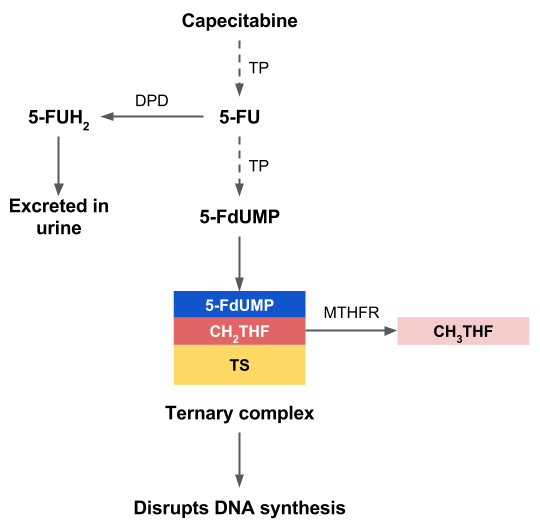
\includegraphics[scale=0.35]{fluorouracil.png}
\end{figure}%
\column{5cm}
\begin{itemize}
\item Exon 14 is skipped, producing an inactive enzyme with no uracil-binding site.
\item Strong clinical evidence indicating association with severe fluoropyrimidine-related toxicity.
\end{itemize}
\end{columns}
\blfootnote{B. Mohelnikova-Duchonova, B. Melichar, and P. Soucek, 2014. World J. Gastroenterol, 20(30): 10316-10330.}
\end{frame}

\begin{frame}
\frametitle{98.0\% of germline variants identified in blood are retained in FFPE tumours}
\vspace{-2mm}
\begin{figure}[t]
  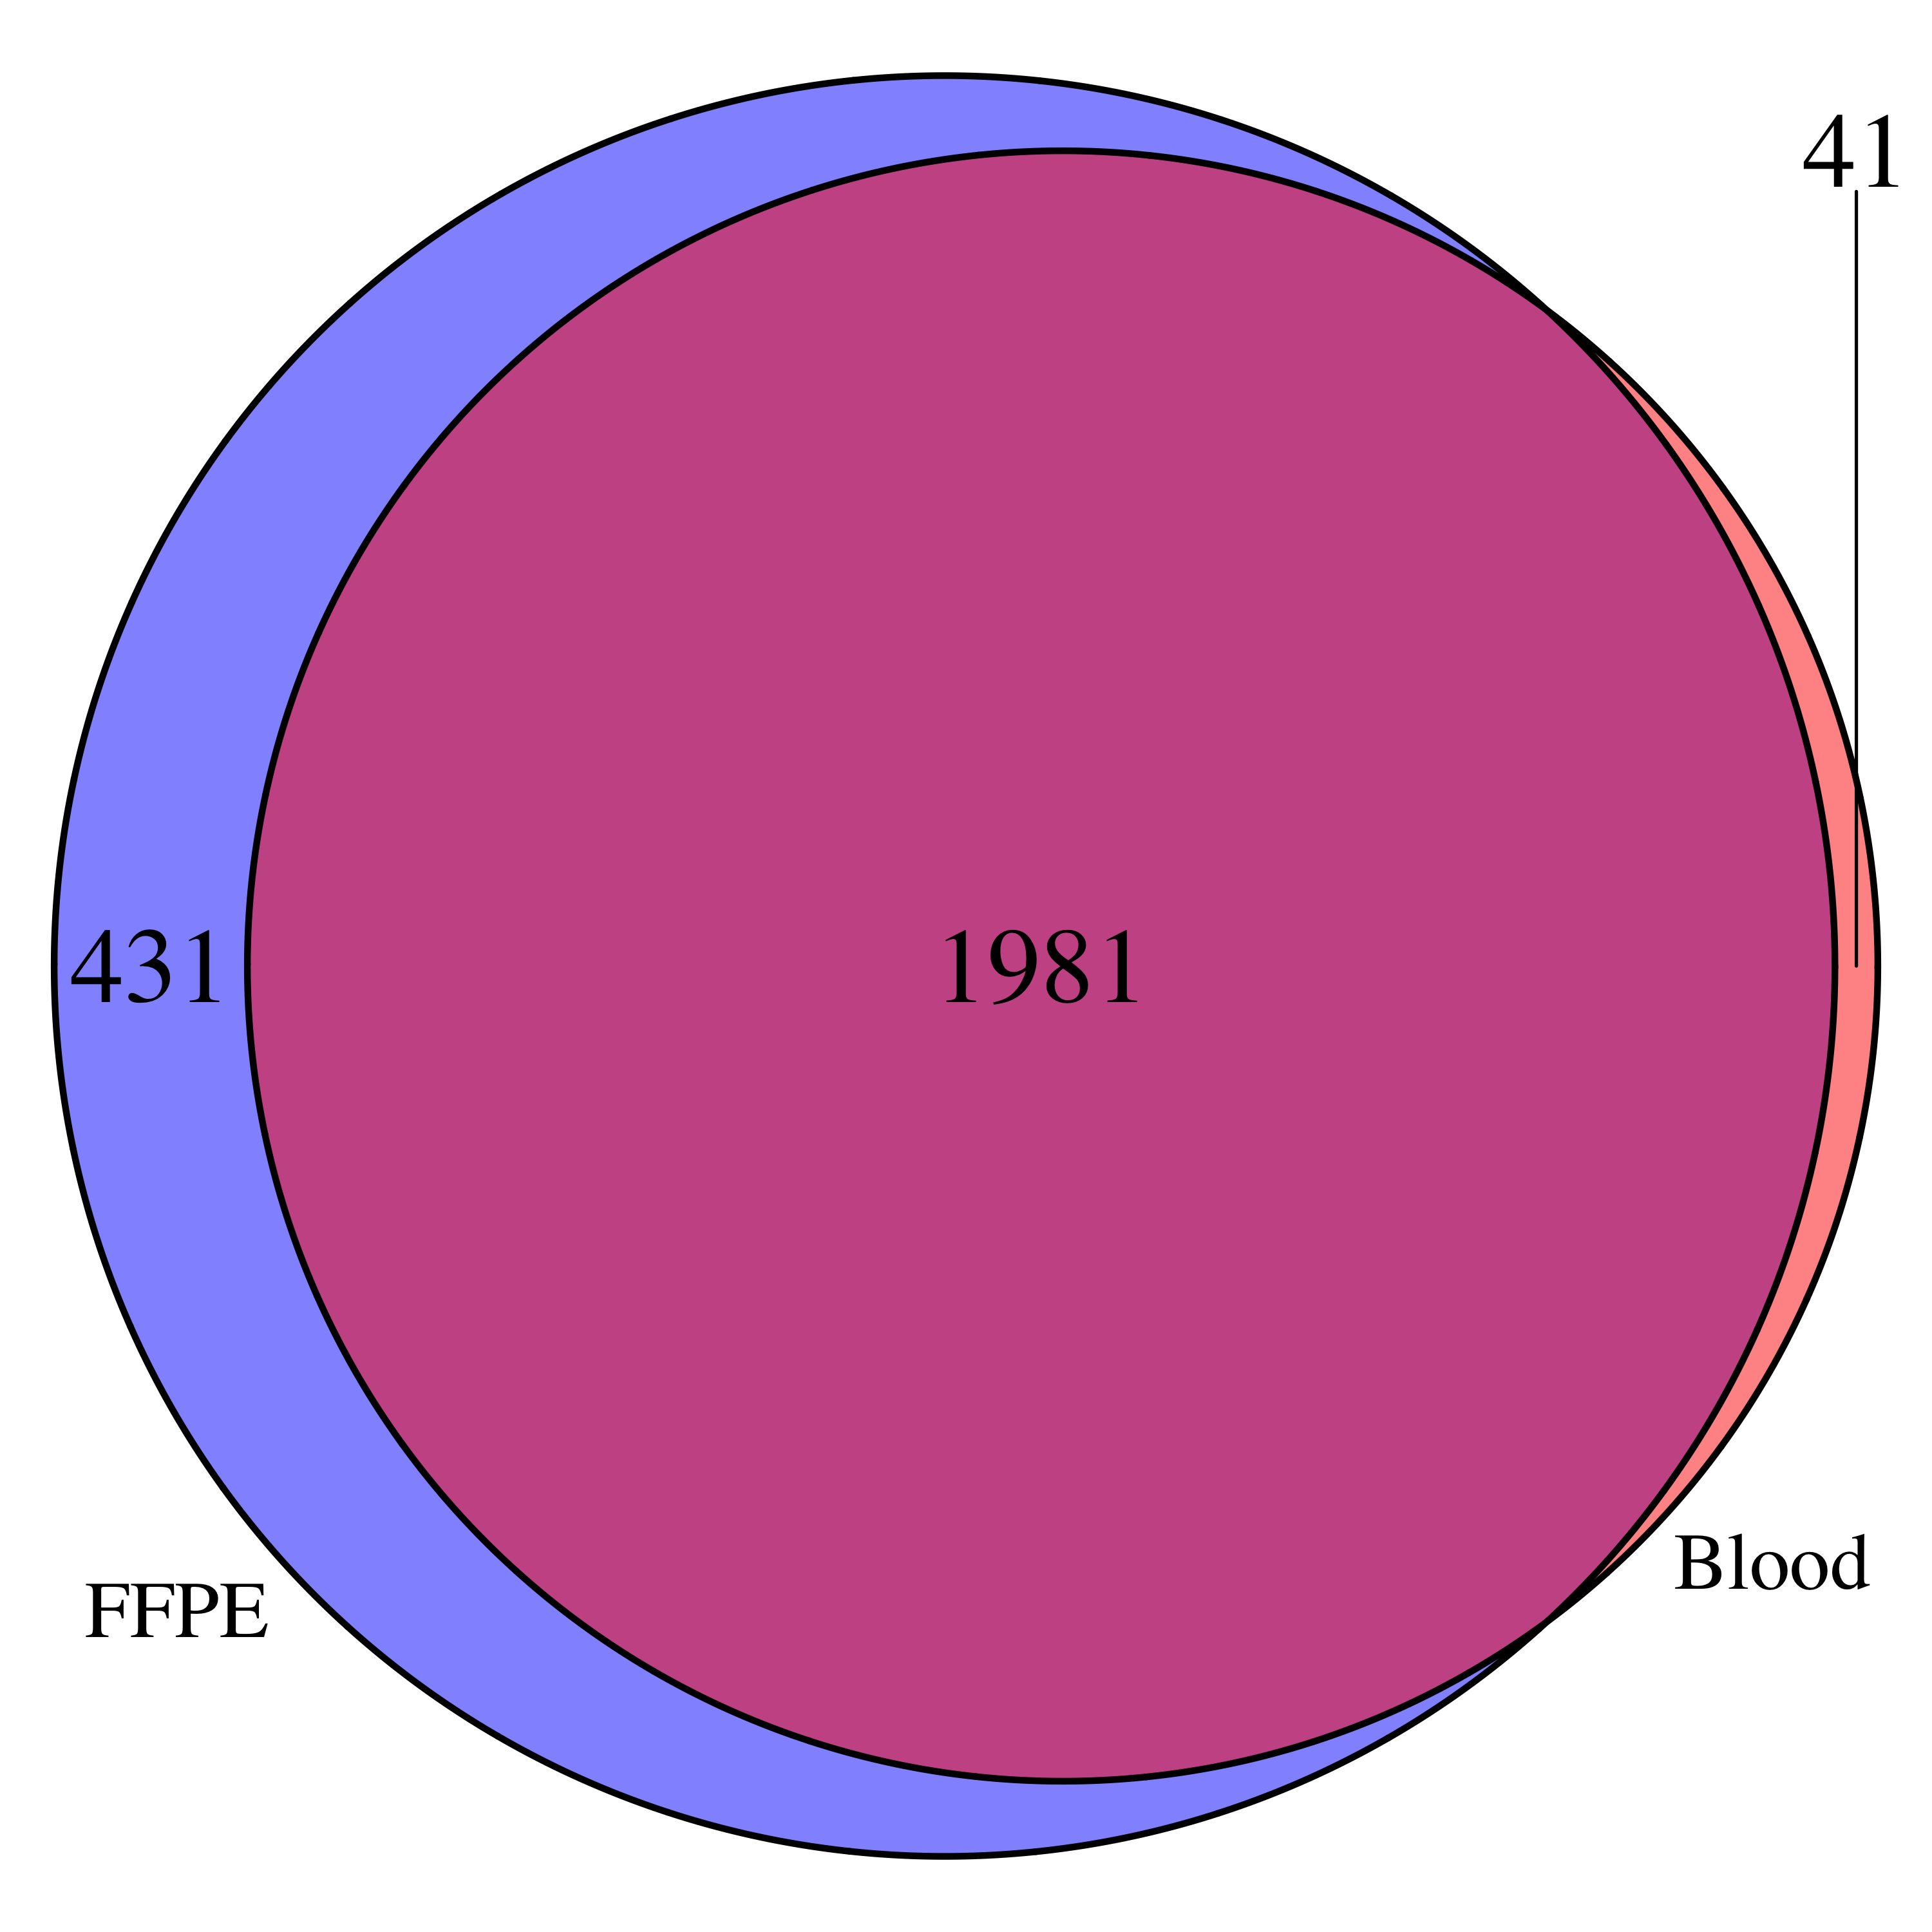
\includegraphics[scale=0.05]{ffpe_blood_conc_venn.png}
\end{figure}
\vspace{-4mm}
\centering
\uncover<2->{\textcolor{blue}{FFPE tumour DNA can be a reliable source \\for germline variant calling.}}
\end{frame}

%%%%%%%%%%%%%%%%%%%%%%%%%%%%%%%%%%%%%%%%%%%%%%%%%%%%%%%%%%%%%%%%%%%%%
% Project Aim 3
\section[Aim 3]{Aim 3: The use of a VAF cut-off could result in high sensitivity in identifying germline variants in FFPE tumours with an acceptable positive predictive value.}
%%%%%%%%%%%%%%%%%%%%%%%%%%%%%%%%%%%%%%%%%%%%%%%%%%%%%%%%%%%%%%%%%%%%%

\begin{frame}
\frametitle{Variant allele frequency (VAF)}
\begin{figure}[t]
    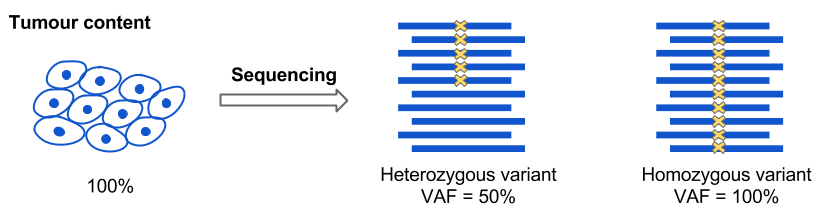
\includegraphics[scale=0.38]{vaf_cells3.png}
\end{figure}
\end{frame}

\begin{frame}
\frametitle{VAF in tumour specimens can deviate from diploid zygosity}
DNA damage induced by formalin (e.g. fragmentation and sequence artifacts)
\begin{figure}[t]
    
\includegraphics[scale=2]{ffpe_blocks.jpeg}
\end{figure}
\end{frame}

\begin{frame}
\frametitle{Somatic VAF in tumour specimens can deviate from diploid zygosity}
Mixture of tumour and normal cells
\begin{figure}[t]
    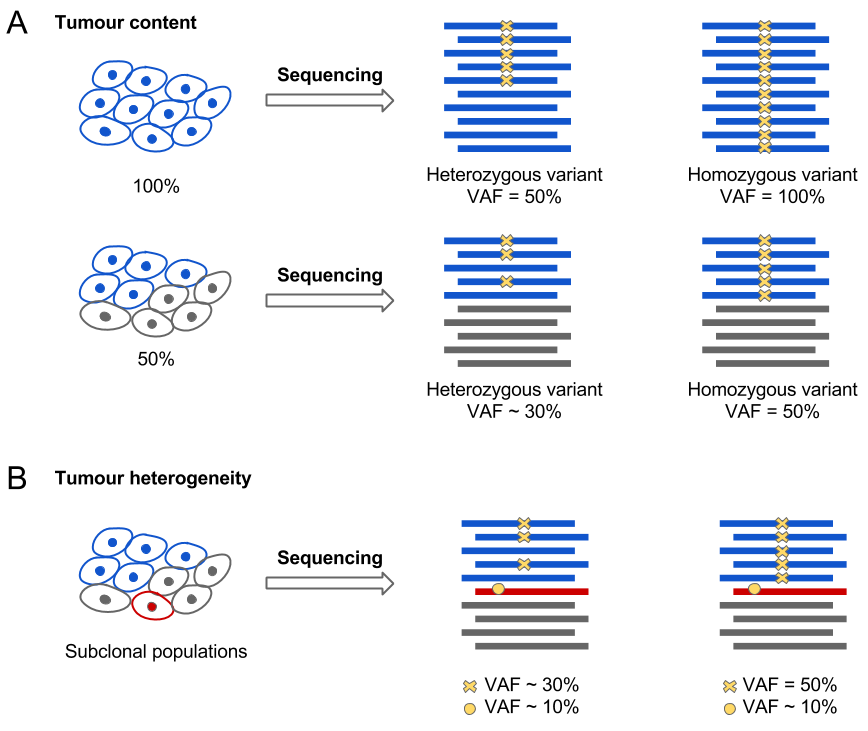
\includegraphics[scale=0.38]{vaf_cells.png}
\end{figure}
\end{frame}

\begin{frame}
\frametitle{Somatic VAF in tumour specimens can deviate from diploid zygosity}
Tumour heterogeneity
\begin{figure}[t]
    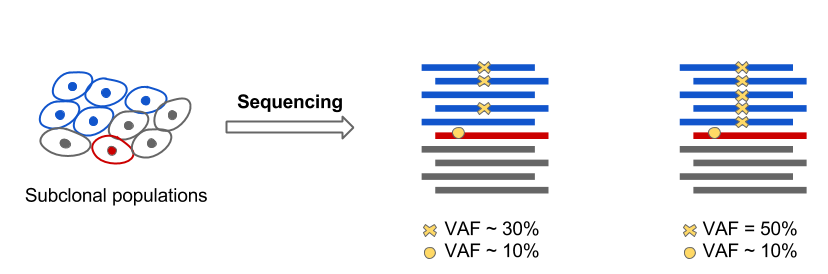
\includegraphics[scale=0.38]{vaf_cells2.png}
\end{figure}
\end{frame}

\begin{frame}
\frametitle{Aim 3: Evaluate the use of VAF thresholds to separate germline from somatic variants in FFPE tumours}
\begin{figure}[t]
    \includegraphics[scale=0.25]{study_design_aim3.png}
\end{figure}
\end{frame}

\begin{frame}
\frametitle{VAF distributions of germline variants are different between blood and FFPE tumours}
\begin{figure}[t]
    \includegraphics[scale=0.6]{germline_sens_minor_no_line3.png}
\end{figure}
\end{frame}

\begin{frame}
\frametitle{Measure sensitivity of identifying germline variants in FFPE tumours}
\begin{figure}[t]
    \includegraphics[scale=0.2]{contingency_table2.png}
\end{figure}
\vspace{-2mm}
\centering
Sensitivity = True positives / (True positives + False negatives)
\end{frame}

\begin{frame}
\frametitle{A VAF cutoff of 15\% would correctly identify 99\% of germline alterations in FFPE tumours}
\centering
\begin{table}
\footnotesize
\centering
      \begin{tabular}{ccc|ll}
        \hline
        VAF (\%) & False Negative & True Positive & Sensitivity & 95\% CI
        \\
        \hline
        10 & 0 & 1981 & 1.0 & 1.0--1.0
        \\
        \textcolor{blue}{15} & \textcolor{blue}{13} & \textcolor{blue}{1968} & \textcolor{blue}{0.99} & \textcolor{blue}{0.99-1.0}
        \\
        20 & 46 & 1935 & 0.98 & 0.97--0.98
        \\
        25 & 77 & 1904 & 0.96 & 0.95--0.97
        \\
        30 & 117 & 1864 & 0.94 & 0.93--0.95
        \\
        35 & 192 & 1789 & 0.90 & 0.89--0.92
        \\
        40 & 313 & 1668 & 0.84 & 0.83--0.86
        \\
        45 & 458 & 1523 & 0.77 & 0.75--0.79
        \\
				\hline
      \end{tabular} \\
\end{table}
\end{frame}

\begin{frame}
\frametitle{Referral of somatic variants to confirmatory germline testing should be minimized}
\begin{figure}[t]
    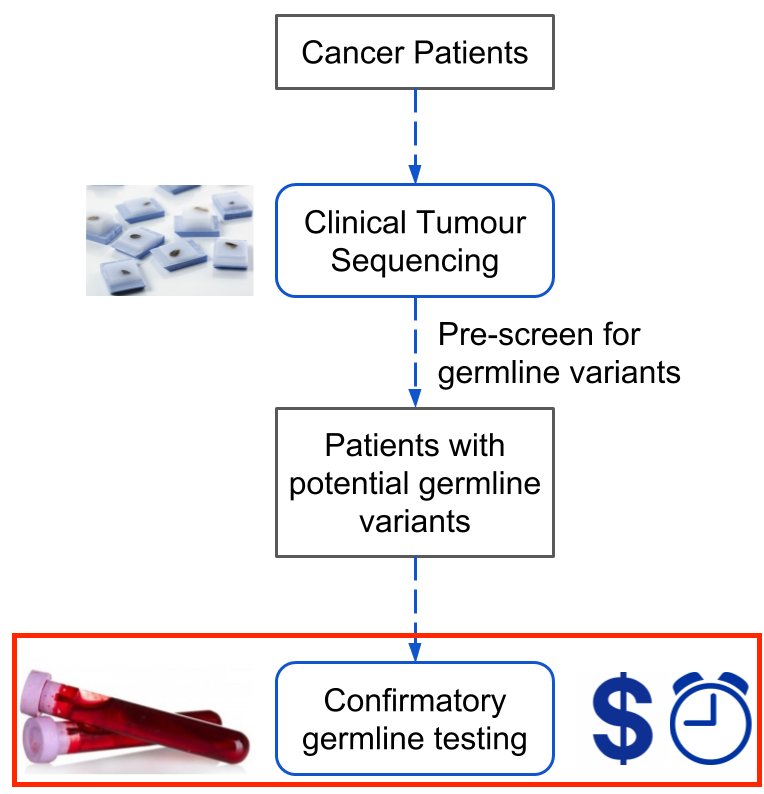
\includegraphics[scale=0.22]{opportunity_clinical_sequencing_research_question2.png}
\end{figure}
\end{frame}

\begin{frame}
\frametitle{VAF distributions are different between germline and somatic variants in FFPE tumours}
\begin{figure}[t]
    \includegraphics[scale=0.6]{germline_ppv_minor_no_line3.png}
\end{figure}
\end{frame}

\begin{frame}
\frametitle{Measure PPVs of identifying germline variants in FFPE tumours for follow-up testing}
\begin{figure}[t]
    \includegraphics[scale=0.2]{contingency_table2.png}
\end{figure}
\vspace{-2mm}
\centering
PPV = True positives / (True positives + False positives)
\end{frame}

\begin{frame}
\frametitle{A VAF cutoff of 15\% would submit 14\% of somatic mutations to follow-up germline testing}
\scriptsize
\begin{table}[H]
\centering
      \begin{tabular}{cccccll}
        \hline
        VAF (\%) & False Positive & True Positive & Total Calls & PPV & 95\% CI
        \\
        \hline
        10 & 431 & 1981 & 2412 & 0.82 & 0.81--0.84
        \\
        \textcolor{blue}{15} & \textcolor{blue}{319} & \textcolor{blue}{1968} & \textcolor{blue}{2287} & \textcolor{blue}{0.86} & \textcolor{blue}{0.85--0.87}
        \\
        20 & 273 & 1935 & 2208 & 0.88 & 0.86--0.89
        \\
        25 & 245 & 1904 & 2149 & 0.89 & 0.87--0.90
        \\
        30 & 203 & 1864 & 2067 & 0.90 & 0.89--0.91
        \\
        35 & 178 & 1789 & 1967 & 0.91 & 0.90--0.92
        \\
        40 & 146 & 1668 & 1814 & 0.92 & 0.91--0.93
        \\
        45 & 118 & 1523 & 1641 & 0.93 & 0.91--0.94
        \\
				\hline
      \end{tabular} \\
\end{table}
\end{frame}

%%%%%%%%%%%%%%%%%%%%%%%%%%%%%%%%%%%%%%%%%%%%%%%%%%%%%%%%%%%%%%%%%%%%%
% Conclusion
\section{Conclusions}
%%%%%%%%%%%%%%%%%%%%%%%%%%%%%%%%%%%%%%%%%%%%%%%%%%%%%%%%%%%%%%%%%%%%%

\begin{frame}
\frametitle{Conclusions}
\begin{enumerate}
\uncover<1->{\item Formalin-induced DNA fragmentation and cytosine deamination were detectable, but the discrepancies were minor and could be mitigated by using shorter amplicons and avoiding long-term storage of FFPE blocks.}
\uncover<2->{\item 98.0\% of germline alterations identified in the blood were retained in the tumours, suggesting that FFPE tumour DNA can be a reliable source for germline variant calling.}
\uncover<3->{\item A VAF cut-off of 15\% would correctly identify 99\% of germline alterations in FFPE tumours, but erroneously submit 14\% of somatic mutations for follow-up germline testing.}
\end{enumerate}
\end{frame}

\begin{frame}
\frametitle{Conclusions}
\begin{enumerate}
\setcounter{enumi}{3}
\uncover<1->{\item This underscores the high sensitivity and positive predictive value of using VAF to discriminate between germline and somatic variants.}
\end{enumerate}
\only<2->{\textcolor{blue}{Collectively, these results demonstrate that clinical tumour amplicon sequencing could also be used to provide cost-efficient first-line germline testing.}}
\end{frame}

%%%%%%%%%%%%%%%%%%%%%%%%%%%%%%%%%%%%%%%%%%%%%%%%%%%%%%%%%%%%%%%%%%%%%
\begin{frame}
\frametitle{Acknowledgements}
\begin{columns}[T] % align columns
\begin{column}{.48\textwidth}
\small
Dr. Aly Karsan \\
Dr. Jennifer Grants \\
Dr. Jeremy Parker \\
Dr. Kieran O'Neill \\
Dr. Marion van den Bosch \\
Dr. Rawa Ibrahim \\
Dr. Sergio Martinez-Hoyer \\
Angela Mo \\
Aparna Gopal \\
Deborah Deng \\
Helen Lin \\
Jenny Li \\
Kristy Dockstader \\
Patrick Coulombe \\
Rod Docking \\
Sukhbir Manku
\end{column}%
\hfill%
\begin{column}{.48\textwidth}
\small
\textbf{Committee members:} \\
Dr. Martin Hirst \\
Dr. Ryan Morin
\\~\\
Centre for Clinical Genomics
\\~\\
Canada's Michael Smith Genome Sciences Centre
\\~\\
\textbf{Funding sources:} \\
Canadian Institutes of Health Research \\
UBC Centre for Blood Research
\\~\\
Patients from The OncoPanel Pilot study (H14-01212)
\end{column}%
\end{columns}
\end{frame}

%Supplementary
%%%%%%%%%%%%%%%%%%%%%%%%%%%%%%%%%%%%%%%%%%%%%%%%%%%%%%%%%%%%%%%%%%%%%
\begin{frame}
\frametitle{Process for evaluation of genetic tests}
\begin{figure}[t]
    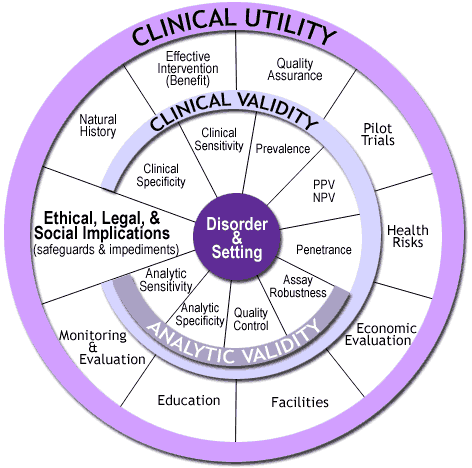
\includegraphics[scale=0.4]{ACCE_wheel.png}
\end{figure}
\end{frame}

%%%%%%%%%%%%%%%%%%%%%%%%%%%%%%%%%%%%%%%%%%%%%%%%%%%%%%%%%%%%%%%%%%%%%
\begin{frame}
\frametitle{Percentage of target bases is significantly different at all coverage thresholds}
\begin{table}
\centering
\tiny
      \begin{tabular}{llllllll}
        \hline
				\multicolumn{1}{l}{ }
				&
				\multicolumn{2}{l}{Blood}
				&&
				\multicolumn{2}{l}{FFPE Tumour}
				&
				\multicolumn{2}{l}{ } \\
				\cline{2-3}\cline{5-6}
        Threshold & Median (\%) & Range (\%) && Median (\%) & Range (\%) & \textit{p} ($<$ 0.05\textsuperscript{*}) & \textit{r}
				\\
				\hline
				$\geq$ 0x & 100.0 & 100.0--100.0 && 100.0 & 97.0--100.0 & 1.0 & 0.068
				\\
				$\geq$ 100x & 100.0 & 100.0--100.0 && 100.0 & 37.0--100.0 & \num{2.3e-4}\textsuperscript{*} & 0.25
				\\
				$\geq$ 200x & 100.0 & 100.0--100.0 && 100.0 & 29.0--100.0 & \num{2.9e-11}\textsuperscript{*} & 0.41
				\\
				$\geq$ 300x & 100.0 & 98.0--100.0 && 99.0 & 24.0--100.0 & \num{4.1e-18}\textsuperscript{*} & 0.55
				\\
				$\geq$ 400x & 99.0 & 94.0--100.0 && 97.0 & 17.0--100.0 & \num{5.0e-28}\textsuperscript{*} & 0.68
				\\
				$\geq$ 500x & 97.0 & 84.0--99.0 && 89.5 & 13.0--99.0 & \num{2.1e-38}\textsuperscript{*} & 0.77
				\\
				$\geq$ 600x & 92.0 & 77.0--97.0 && 87.0 & 9.0--96.0 & \num{1.5e-32}\textsuperscript{*} & 0.72
				\\
				$\geq$ 700x & 84.0 & 70.0--91.0 && 80.0 & 6.0--91.0 & \num{5.7e-25}\textsuperscript{*} & 0.65
				\\
				$\geq$ 800x & 77.0 & 63.0-84.0 && 73.0 & 5.0--83.0 &  \num{4.7e-27}\textsuperscript{*} & 0.67
				\\
				$\geq$ 900x & 73.0 & 54.0--78.0 && 66.0 & 4.0--77.0 &  \num{4.6e-40}\textsuperscript{*} & 0.78
				\\
				$\geq$ 1000x & 68.5 & 41.0--73.0 && 59.0 & 3.0-74.0 & \num{3.6e-42}\textsuperscript{*} & 0.79
				\\
				\hline
      \end{tabular} \\
\end{table}
\end{frame}

%%%%%%%%%%%%%%%%%%%%%%%%%%%%%%%%%%%%%%%%%%%%%%%%%%%%%%%%%%%%%%%%%%%%%
\begin{frame}
\frametitle{Amplicon length and GC content}
\begin{figure}[t]
    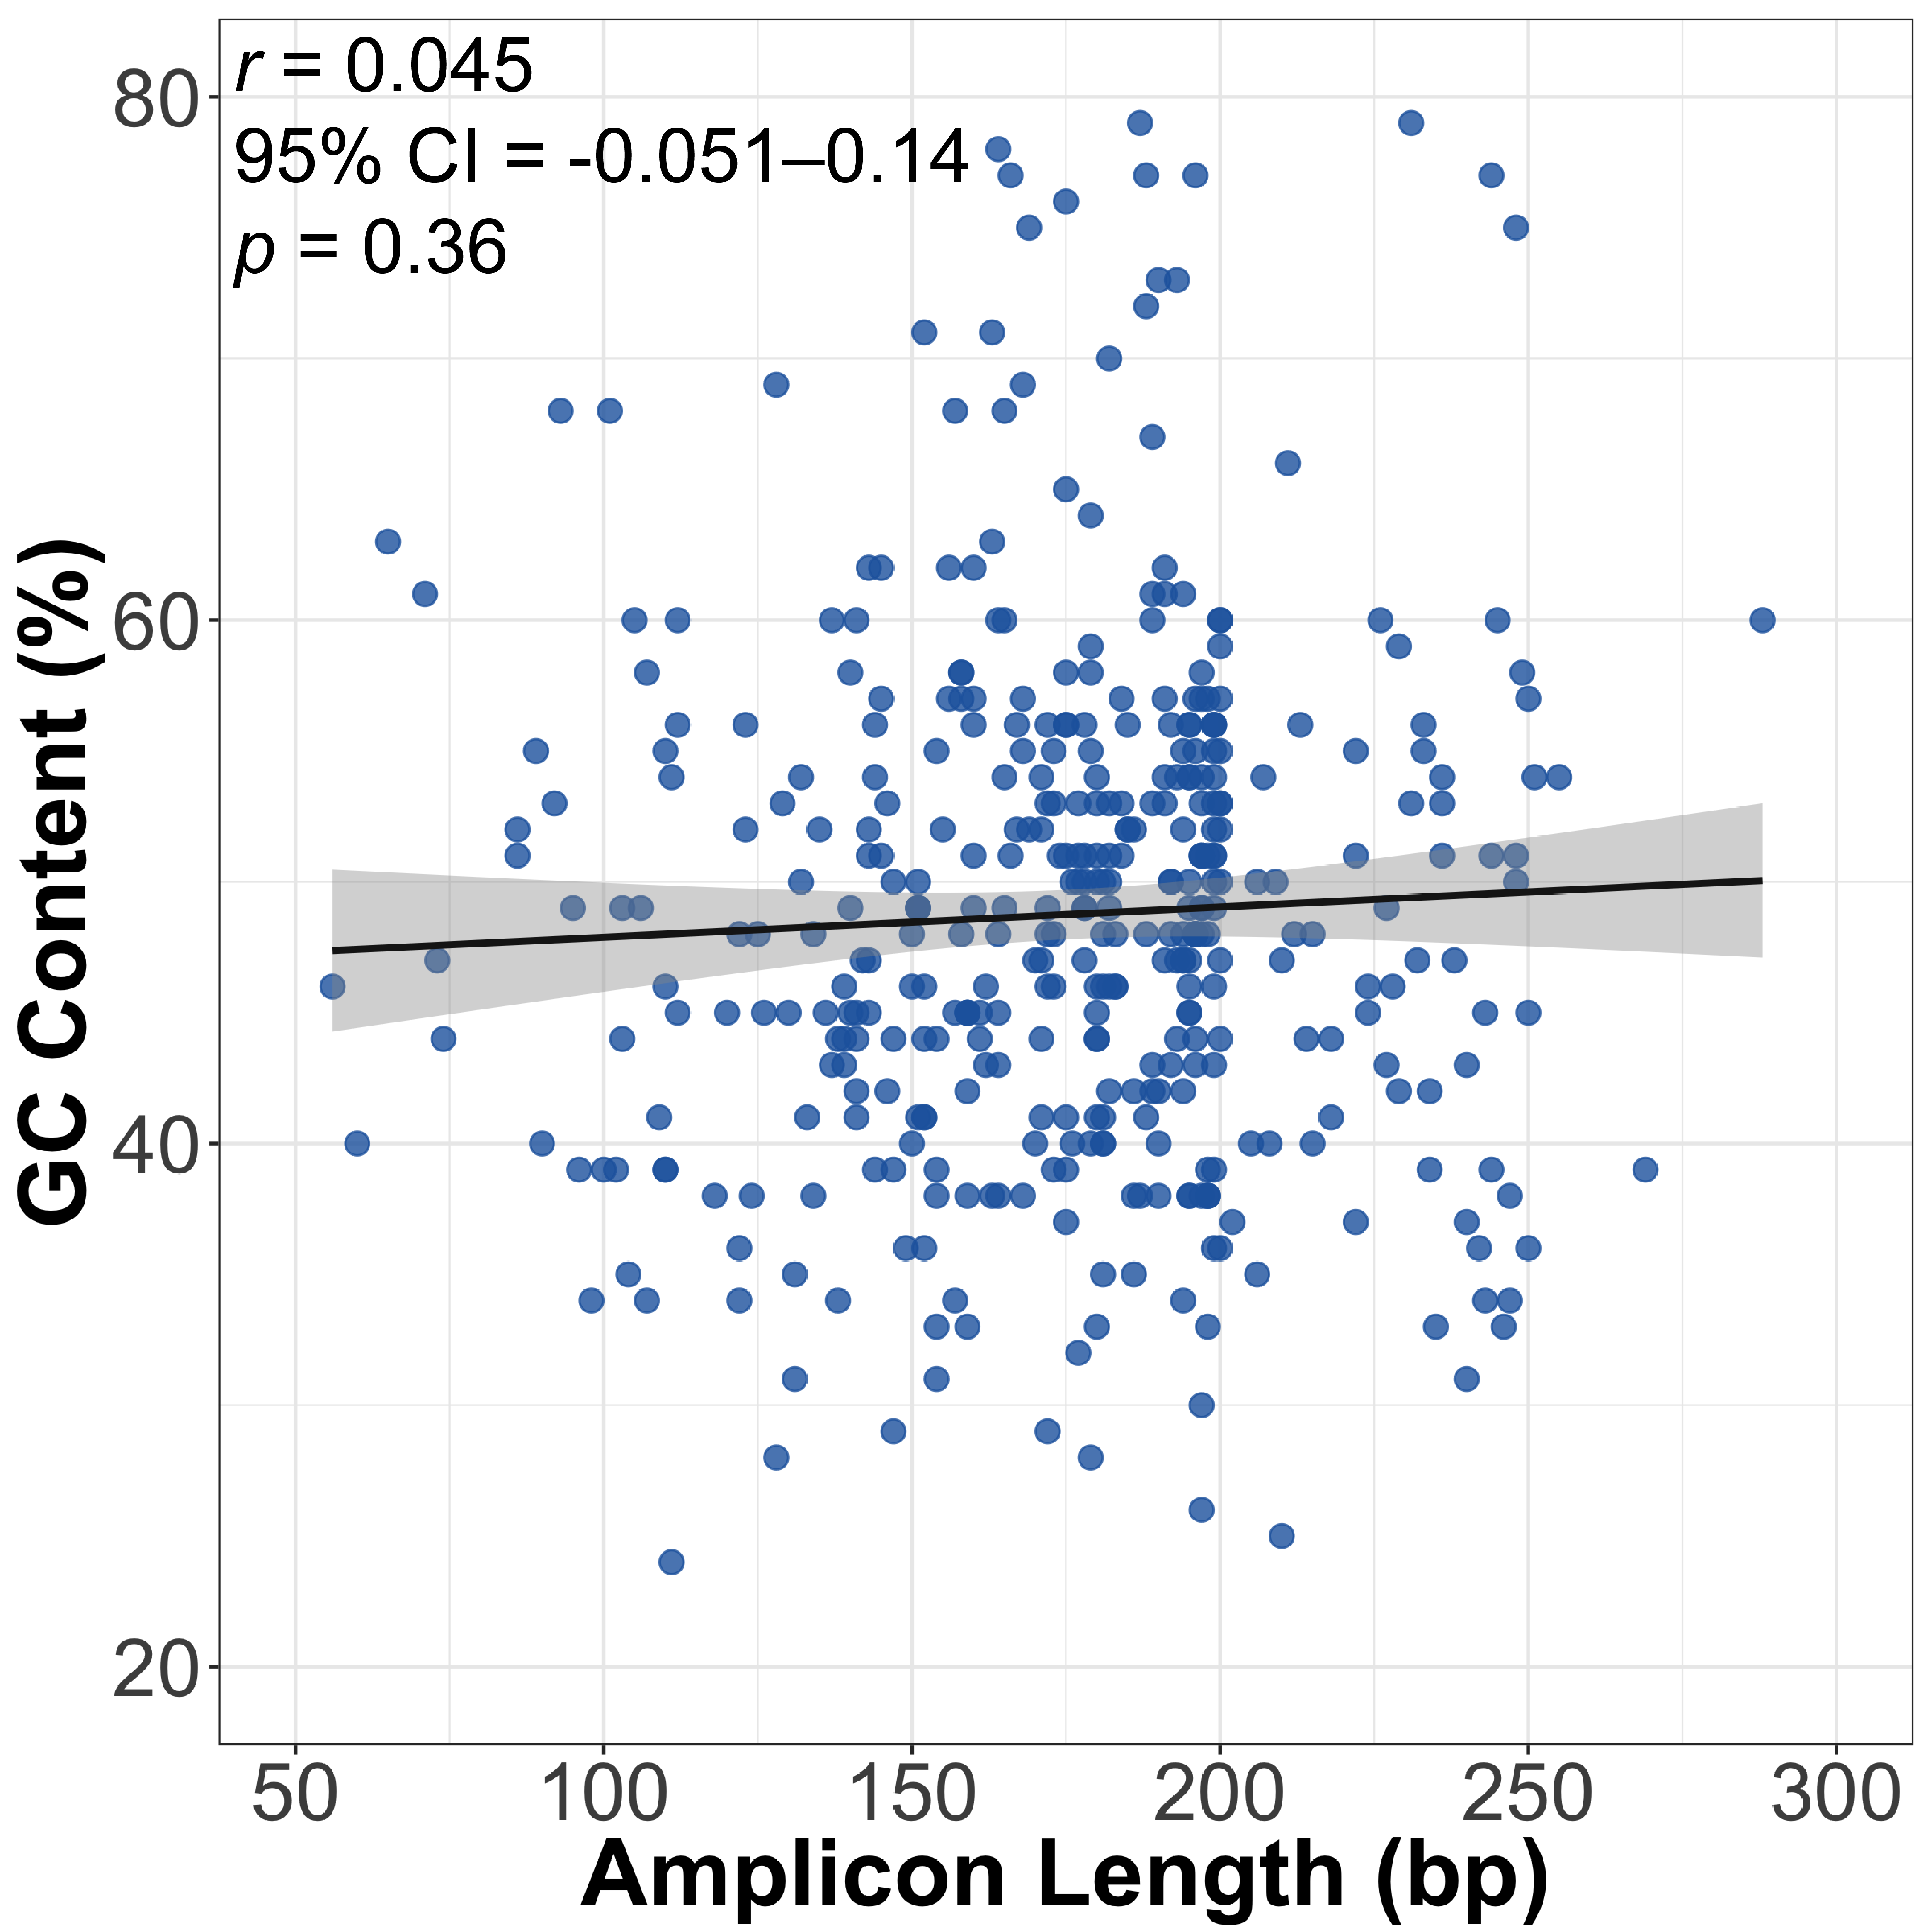
\includegraphics[scale=0.08]{amp_gc_length.png}
    \caption{\scriptsize Pearson's correlation, \textit{p} $<$ 0.05}
\end{figure}
\end{frame}

%%%%%%%%%%%%%%%%%%%%%%%%%%%%%%%%%%%%%%%%%%%%%%%%%%%%%%%%%%%%%%%%%%%%%
\begin{frame}
\frametitle{FFPE specimens demonstrate increased C$>$T/G$>$A sequence artifacts}
\begin{figure}[t]
    \includegraphics[scale=0.58]{deamination_effect_blood_ffpe3.png}
\end{figure}
\end{frame}

%%%%%%%%%%%%%%%%%%%%%%%%%%%%%%%%%%%%%%%%%%%%%%%%%%%%%%%%%%%%%%%%%%%%%
\begin{frame}
\frametitle{FFPE specimens demonstrate increased C$>$T/G$>$A sequence artifacts at low-allelic fraction}
\begin{figure}[t]
    \includegraphics[scale=0.4]{deamination_effect_af_range_3.png}
    \caption{\scriptsize Kruskal-Wallis test, \textit{p} $<$ 0.0001}
\end{figure}
\end{frame}

%%%%%%%%%%%%%%%%%%%%%%%%%%%%%%%%%%%%%%%%%%%%%%%%%%%%%%%%%%%%%%%%%%%%%
\begin{frame}
\frametitle{VAF distributions of germline variants are different between blood and FFPE tumours}
\begin{figure}[t]
    \includegraphics[scale=0.6]{germline_sens_minor_no_line2.png}
\end{figure}
\end{frame}


%%%%%%%%%%%%%%%%%%%%%%%%%%%%%%%%%%%%%%%%%%%%%%%%%%%%%%%%%%%%%%%%%%%%%
\begin{frame}
\frametitle{VAF distributions are different between germline and somatic variants in FFPE tumours}
\begin{figure}[t]
    \includegraphics[scale=0.6]{germline_ppv_minor_no_line2.png}
\end{figure}
\end{frame}

\end{document}



\endinput
%%%%%%%%%%%%%%%%%%%%%%%%%%%%%%%%%%%%%%%%%%%%%%%%%%%%%%%%%%%%%%%%%%%%%
\begin{frame}
\frametitle{Future directions}
\end{frame}

%%%%%%%%%%%%%%%%%%%%%%%%%%%%%%%%%%%%%%%%%%%%%%%%%%%%%%%%%%%%%%%%%%%%%
\begin{frame}
\frametitle{Recap}
\begin{enumerate}
\uncover<1->{\item Tumour sequencing has been rapidly integrated into clinical practice to guide oncologic care.}
\uncover<2->{\item Clinical laboratories are faced with financial, time, and logistical constraints.}
\uncover<3->{\item Tumour genomes may contain both somatic and germline variants.}
\uncover<4->{\item Germline variants have clinical implications for patients and their families.}
\uncover<5->{\item Clinical tumour sequencing presents an opportunity to pre-screen for germline variants.}
\\~\\
\centering
\uncover<6->{\textcolor{blue}{Research question: Can we leverage clinical tumour sequencing for identification of germline variants?}}
\end{enumerate}
\end{frame}

\begin{frame}
\frametitle{Precision oncology: Right cancer treatment, right patient, right dose, right time}
\centering
\begin{figure}[t]
    \includegraphics[scale=0.3]{precision_oncology.png}
\end{figure}
\blfootnote{S. Roychowdhury \& A.M. Chinnaiyan, 2014. Annu. Rev. Genomics Hum. Genet, 15:395-415}
\end{frame}

\begin{frame}
\frametitle{Guiding principles of precision oncology}
\begin{figure}[t]
    \includegraphics[scale=0.32]{precision_oncology_timeline1.png}
\end{figure}
\blfootnote{L.A. Garraway, 2013. J. Clin. Oncol, 31(15):1805-1814}
\end{frame}

\begin{frame}
\frametitle{Guiding principles of precision oncology}
\begin{figure}[t]
    \includegraphics[scale=0.32]{precision_oncology_timeline2.png}
\end{figure}
\blfootnote{L.A. Garraway, 2013. J. Clin. Oncol, 31(15):1805-1814}
\end{frame}

\begin{frame}
\frametitle{Guiding principles of precision oncology}
\begin{figure}[t]
    \includegraphics[scale=0.32]{precision_oncology_timeline3.png}
\end{figure}
\blfootnote{L.A. Garraway, 2013. J. Clin. Oncol, 31(15):1805-1814}
\end{frame}

\begin{frame}
\frametitle{Guiding principles of precision oncology}
\begin{figure}[t]
    \includegraphics[scale=0.32]{precision_oncology_timeline4.png}
\end{figure}
\blfootnote{L.A. Garraway, 2013. J. Clin. Oncol, 31(15):1805-1814}
\end{frame}

\begin{frame}
\frametitle{Guiding principles of precision oncology}
\begin{figure}[t]
    \includegraphics[scale=0.32]{precision_oncology_timeline5.png}
\end{figure}
\blfootnote{L.A. Garraway, 2013. J. Clin. Oncol, 31(15):1805-1814}
\end{frame}

\begin{frame}
\frametitle{Guiding principles of precision oncology}
\begin{figure}[t]
    \includegraphics[scale=0.32]{precision_oncology_timeline6.png}
\end{figure}
\blfootnote{L.A. Garraway, 2013. J. Clin. Oncol, 31(15):1805-1814}
\end{frame}

\begin{frame}
\frametitle{Limitations in clinical laboratories that offer genomic tests}
\begin{enumerate}
\uncover<1->{\item \textcolor{blue}{Cost}: Healthcare resources must be allocated reasonably and efficiently.}
\uncover<2->{\item \textcolor{blue}{Turnaround time}: Genomic reports must be returned within a reasonable time frame.}
\uncover<3->{\item \textcolor{blue}{Logistical}: Sample collection and storage must be thoroughly maintained.}
\\~\\
\centering
\uncover<4->{\textcolor{blue}{90\% of tumours are sequenced in clinical practice without matched normal samples.}}
\end{enumerate}
\end{frame}

\begin{frame}
\frametitle{Tumour genomes may contain both germline and somatic variants}
\begin{figure}[t]
    \includegraphics[scale=0.3]{somatic_germline_tumour1.png}
\end{figure}
\end{frame}

\begin{frame}
\frametitle{Tumour genomes may contain both germline and somatic variants}
\begin{figure}[t]
    \includegraphics[scale=0.3]{somatic_germline_tumour2.png}
\end{figure}
\end{frame}

\begin{frame}
\frametitle{Germline variants can have clinical implications for both cancer patients and their families}
\begin{figure}[t]
    \includegraphics[scale=0.28]{germline_importance.png}
\end{figure}
\end{frame}

\begin{frame}
\frametitle{Clinical tumour sequencing presents an opportunity to pre-screen for germline variants}
\begin{figure}[t]
    \includegraphics[scale=0.2]{opportunity_to_prescreen1.png}
\end{figure}
\end{frame}

\begin{frame}
\frametitle{Clinical tumour sequencing presents an opportunity to pre-screen for germline variants}
\begin{figure}[t]
    \includegraphics[scale=0.2]{opportunity_to_prescreen2.png}
\end{figure}
\end{frame}

\begin{frame}
\frametitle{Clinical tumour sequencing presents an opportunity to pre-screen for germline variants}
\begin{figure}[t]
    \includegraphics[scale=0.2]{opportunity_to_prescreen3.png}
\end{figure}
\end{frame}

% Supplementary
%%%%%%%%%%%%%%%%%%%%%%%%%%%%%%%%%%%%%%%%%%%%%%%%%%%%%%%%%%%%%%%%%%%%%
\begin{frame}
\frametitle{Supplementary Figures and Tables}
\end{frame}

\begin{frame}
\frametitle{Amplicon length and GC content}
\begin{figure}[t]
    \includegraphics[scale=0.08]{amp_gc_length.png}
\end{figure}
\end{frame}

\begin{frame}
\frametitle{Precision oncology}
\begin{figure}[t]
    \includegraphics[scale=0.7]{somatic_precision.png}
\end{figure}
\end{frame}

%%%%%%%%%%%%%%%%%%%%%%%%%%%%%%%%%%%%%%%%%%%%%%%%%%%%%%%%%%%%%%%%%%%%%
\begin{frame}
\frametitle{Deamination effects lead to increased C$>$T/G$>$A transitions in FFPE specimens (Wilcoxon signed-rank test)}
\begin{figure}[t]
    \includegraphics[scale=0.58]{deamination_effect.png}
\end{figure}
\end{frame}

%%%%%%%%%%%%%%%%%%%%%%%%%%%%%%%%%%%%%%%%%%%%%%%%%%%%%%%%%%%%%%%%%%%%%
\begin{frame}
\frametitle{Deamination effects lead to increased C$>$T/G$>$A transitions in FFPE specimens (Wilcoxon signed-rank test, fold change)}
\begin{figure}[t]
    \includegraphics[scale=0.58]{deamination_effect_blood_fc.png}
\end{figure}
\end{frame}

%%%%%%%%%%%%%%%%%%%%%%%%%%%%%%%%%%%%%%%%%%%%%%%%%%%%%%%%%%%%%%%%%%%%%
\begin{frame}
\frametitle{Deamination effects lead to increased C$>$T/G$>$A transitions in FFPE specimens at low allele frequency (Wilcoxon signed-rank test)}
\begin{figure}[t]
    \includegraphics[scale=0.4]{deamination_effect_af_range.png}
\end{figure}
\end{frame}

\begin{frame}
\frametitle{Correlation between DNA input and amplicon yield}
\begin{figure}[t]
    \begin{columns}
    \column{7cm}
    \centering
    \includegraphics[scale=0.7]{dna_input_amp_yield.png}%
    \column{5cm}
    \centering
    Enrichment efficiency:
    \[
    log2\frac{\text{Amplicon Yield}}{\text{DNA Input}}
    \]
    \end{columns}
\end{figure}
\end{frame}

\begin{frame}
\begin{table}
\caption{Determination of correlation between pre-sequencing variables and sequencing results using Spearman's correlation. Top values represent Spearman's \textit{rho} and 95\% confidence interval in brackets, whereas bottom values represent \textit{p}-value. Asterisk(*) indicates significance level of \textit{p}-value $<$ 0.05.}
\tiny
\centering
      \begin{tabular}{l|l|l|l|ll}
        Variable & Amplicon & Age of Paraffin & Fraction of & Average Per Base
        \\
				 & Yield (ng) & Block (Day) & C$>$T/G$>$A & Normalized Coverage
				\\
        \hline
        Age of Paraffin & -0.42 (-0.52-- -0.30) & & &
				\\
				Block (Day) & \num{5.2e-7}\mbox{*} & & &
        \\
				\hline
				Fraction of & -0.72 (-0.77-- -0.65) & 0.54 (0.61--0.75) & &
				\\
				C$>$T/G$>$A & \num{1.9e-11}\mbox{*} & \num{6.3e-35}\mbox{*} & &
				\\
				\hline
				Average Per Base & 0.69 (0.61--0.75) & -0.47 (-0.57-- -0.36) & -0.80 (-0.84-- -0.75) &
				\\
				Normalized Coverage & \num{8.5e-20}\mbox{*} & \num{4.7e-7}\mbox{*} & \num{7.5e-17}\mbox{*} &
				\\
				\hline
				On-target & 0.58 (0.48--0.66) & -0.35 (-0.46-- -0.23) & -0.57 (-0.65-- -0.47) & 0.73 (0.66--0.79)
				\\
				Aligned Reads (\%) & \num{2.1e-13}\mbox{*} & \num{8.2e-3}\mbox{*} & \num{4.2e-8}\mbox{*} & \num{3.1e-58}\mbox{*}
				\\
				\hline
      \end{tabular} \\
\end{table}
\end{frame}
